%Kompiliuoti su XeLaTeX ir BibTeX

\documentclass[a4paper, 12pt]{article}

\usepackage[yyyymmdd]{datetime}

\usepackage{fontspec}
\usepackage{fontenc}
\usepackage{ulem}
\usepackage{cite}
\usepackage{mathtools}
\usepackage{amsmath}
\usepackage{amssymb}
%\usepackage{float}
\usepackage{graphicx}
\usepackage{multirow}
\usepackage[hyphens]{url}
\usepackage{caption}
\usepackage[svgnames]{xcolor}
\usepackage{lineno}
\usepackage[lithuanian]{babel}
\usepackage{hyperref}
\usepackage{siunitx}
\usepackage{floatrow}

\floatsetup[table]{capposition=top}

\hypersetup{breaklinks=true}
\urlstyle{same}

\usepackage{geometry}
\pagestyle{myheadings}
\geometry{
	left=3cm,
	right=1cm,
	top=2cm,
	bottom=2cm,
}
\pagenumbering{arabic}
\linespread{1.25}

\graphicspath{ {images/} }

\renewcommand{\dateseparator}{-}
\addto\captionslithuanian{\renewcommand{\figurename}{pav}}
\addto\captionslithuanian{\renewcommand{\refname}{Literatūros sąrašas}}
\addto\captionslithuanian{\renewcommand{\tablename}{lentelė}}

\DeclareCaptionLabelFormat{numfirst}{#2~#1}
\captionsetup[figure]{labelformat = numfirst, labelsep = period}
\captionsetup[table]{labelformat = numfirst, labelsep = period}

\newcommand{\textblue}[1]{{\color{Blue}#1}}
\newcommand{\textred}[1]{{\color{Red}#1}}
\newcommand{\comment}[1]{\newline\textblue{#1}\newline}
\newcommand{\commentNL}[1]{\textblue{#1}\newline}
\newcommand{\commentMA}[1]{\textred{#1}\newline}
\newcommand{\ttt}[1]{\texttt{#1}}
\newcommand{\pT}{p_{\mathrm{T}}}
\newcommand{\ET}{E_{\mathrm{T}}}
\newcommand{\WW}{W\! W}
\newcommand{\ZZ}{Z\! Z}
\newcommand{\WZ}{W\! Z}
\newcommand{\tbarW}{\bar{t}W}
\newcommand{\ttbar}{t\bar{t}}
\newcommand{\emu}{e\mu}
\newcommand{\mumu}{\mu\mu}
\newcommand{\gJets}{\gamma\! +\!\mathrm{Jets}}
\newcommand{\WJets}{W\! +\!\mathrm{Jets}}
\newcommand{\dtW}{tW\! + \! \bar{t}W}
\newcommand{\DYee}{\mathrm{DY} \! \rightarrow \! ee}
\newcommand{\DYtau}{\mathrm{DY} \! \rightarrow \! \tau\tau}
\newcommand{\DY}{\mathrm{DY}}
\newcommand{\ltq}[1]{{\quotedblbase{}#1\textquotedblleft{}}}
\newcommand{\Lumi}{{\cal L}_\mathrm{int}}
\newcommand{\invfb}{fb$^{-1}$}
\newcommand{\invpb}{pb$^{-1}$}
\newcommand{\QCD}{QC\! D}

\newlength\q
\setlength\q{\dimexpr .5\textwidth -2\tabcolsep}

\begin{document}
%\linenumbers

\begin{titlepage}
\centering
{\large Vilniaus universitetas \\ Fizikos fakultetas \\ Teorinės fizikos ir astronomijos institutas \par}
\vspace{3.5cm}
{\Large Marijus Ambrozas \par}
\vspace{0.3cm}
{\Large Drell-Yan proceso tyrimas analizuojant CERN CMS eksperimento 2016 metų protonų susidūrimų duomenis \par}
\vspace{0.8cm}
{\large Magistrantūros studijų mokslo tiriamasis darbas \par}
\vspace{0.8cm}
{\large Teorinės fizikos ir astrofizikos \\ studijų programa \par}
\vspace{3.5cm}
{\large \begin{tabular*}{0.9\textwidth}{@{\extracolsep{\fill}}ll}
Studentas & Marijus Ambrozas\tabularnewline[0.5cm]
Darbo vadovas & dr. Andrius Juodagalvis\tabularnewline[0.5cm]
Instituto atstovas & prof. Egidijus Anisimovas\tabularnewline[0.5cm]
\end{tabular*} \par}
\vspace{4cm}
{\large Vilnius $2019$\par}
\end{titlepage}


\clearpage
\addtocounter{page}{1}
\addtocontents{toc}{\protect\setcounter{tocdepth}{2}}
\tableofcontents
\clearpage

\section*{Įvadas} \addcontentsline{toc}{section}{Įvadas}

Didelės energijos subatominių dalelių susidūrimai, vykdomi CERN Didžiajame hadronų greitintuve
(angl.\ \textit{Large Hadron Collider} -- LHC), suteikia galimybę pažvelgti į mažiausius
Visatos statybinius blokus bei jų tarpusavio sąveikas, taip pat, ieškoti atsakymų į dar
neatsakytus fizikinius klausimus ir tikrinti naujas teorijas.
Stengiantis surinkti kuo daugiau informacijos apie labai retai įvykstančius
dalelių sąveikos procesus, greitintuve yra didinamas registruojamų protonų susidūrimų
skaičius: pavyzdžiui, per 2016 metus buvo užregistruota maždaug 10 kartų daugiau protonų
susidūrimų, nei per 2015 metus.
Tai sudaro nemažą iššūkį mokslininkams, kurie turi nuspręsti, kur reikia saugoti
didžiulius kiekius duomenų ir kaip sumažinti jų analizės trukmę.

Norint geriau suprasti tai, kas buvo užregistruota protonų susidūrimus
fiksuojančiuose detektoriuose, labai svarbu turėti kaip įmanoma tikslesnį protonų
tarpusavio sąveikos bei jų sandaros aprašymą.
Tokiu būdu galima lyginti teoriškai numatomus rezultatus su užregistruotaisiais eksperimento
metu.
Teorinėje dalelių fizikoje protonų sandara aprašoma partonų pasiskirstymo funkcijomis
(angl.\ \textit{parton distribution functions} -- PDF), nuo kurių tikslumo priklauso teorinių
įverčių kokybė.
Kvantinės chromodinamikos teorijos bei elektrosilpnosios sąveikos teorijų tobulinimui nemažą
svarbą turi eksperimentinis Drell-Yan proceso tyrimas.
Tikslūs Drell-Yan diferencialinio reakcijos skerspjūvio matavimai leidžia tikslinti partonų
pasiskirstymo funkcijas bei palengvina kitus eksperimentinės didelių energijų fizikos tyrimus,
kur Drell-Yan procesas yra dominuojantis triukšmas.

Vis dėlto, didelis duomenų kiekis nėra vienintelis sunkumas šio proceso tyrime -- eksperimentiniai
duomenys visada būna užteršti triukšmo įvykių, kurių indėlį į gaunamą rezultatą reikia įvertinti.
Neretai triukšmo įvykių skaičiaus įvertinimui vien kompiuterinio modeliavimo nepakanka.
Tokiais atvejais į pagalbą pasitelkiami matavimu grįsti metodai.
Tam tikrų Drell-Yan triukšmo procesų įvykių skaičių galima įvertinti $\emu$ metodu.
Šio darbo tikslas -- iš didelės apimties pirminio duomenų rinkinio atrinkti su Drell-Yan
procesu siejamus protonų susidūrimo įvykius, bei $\emu$ metodu įvertinti, kokią atrinktų
duomenų rinkinio dalį užima triukšmo įvykiai.
Šiam tikslui įgyvendinti buvo naudojami 2016 metais CERN CMS detektoriaus užregistruoti $13$
TeV energijos protonų susidūrimų duomenys.

\clearpage

\section{Drell-Yan procesas ir jo tyrimas}

Šiame skyriuje bus trumpai aptariama protonų sandara, pristatomas Drell-Yan procesas,
jo svarba, supažindinama, su kokiomis fizikinėmis sąvokomis ir dydžiais dažnai susiduriama,
kai kalbama apie šį procesą.
Taip pat bus pasakojama apie eksperimentinius didelių energijų fizikos tyrimus, Didįjį hadronų
greitintuvą ir Kompaktiškąjį miuonų solenoidą (angl.\ \textit{Compact Muon Solenoid} -- CMS),
bei apie esmines Kompaktiškojo miuonų solenoido eksperimente vykdomų fizikinių procesų tyrimų
specifikas, supažindinama su didelių energijų fizikos duomenų analizės pagrindais.


\subsection{Protono sandara ir Drell-Yan procesas}


\subsubsection{Partonų pasiskirstymo funkcijos}

Teorinėje elementariųjų dalelių fizikoje protonų, kaip ir kitų hadronų, sandara aprašoma
jų sudedamųjų dalių, vadinamų partonais, pasiskirstymo funkcijomis.
Tikslus šių funkcijų žinojimas yra ypatingai svarbus norint teoriškai aprašyti bet kokius
hadronų greitintuvuose vykstančius procesus.
Partonų pasiskirstymo funkcija $f_{i}(x, Q^{2})$ aprašo tikimybę aptikti protono impulso
dalį $x$ nešantį $i$ tipo partoną (pavyzdžiui, kylantįjį kvarką -- $u$, krentantįjį
kvarką -- $d$ ir t.t.), kai \textit{kietojo} susidūrimo (angl.\ \textit{hard interaction} --
procesas, kurio metu smarkiai pasikeičia dalelių impulsas) energija lygi $Q$.
Du partonų pasiskirstymo funkcijų pavyzdžiai, esant skirtingoms susidūrimų energijoms, yra pateikti
\ref{fig:PDFs} paveiksle.

\medskip
Teoriniai dviejų protonų susidūrimo metu galimų reakcijų skerspjūviai yra apskaičiuojami kaip
partonų pasiskirstymo funkcijų ir partonų tarpusavio reakcijos skerspjūvio kombinacija:

\medskip
\begin{equation}
	\sigma = \sum_{i, j} \int \mathrm{d}x_1 \int \mathrm{d}x_2 \,
	f_{i}(x_1, \, Q^2) \, f_{j}(x_2 \, Q^2) \, \hat{\sigma}(x_1 p_1, \, x_2 p_2, \, Q^2) \; \mathrm{,}
	\label{eq:PDFxsec}
\end{equation}
čia $\sigma$ -- reakcijos skerspjūvis, $i$, $j$ -- sąveikaujantys partonai, nešantys protonų impulsų $p_1$ ir $p_2$
dalis $x_1$ ir $x_2$, o $f_{i}(x_1, \, Q^2)$ ir $f_{j}(x_2, \, Q^2)$ -- partonų pasiskirstymo funkcijos, kai
reakcijos metu perduodama energija lygi $Q$.

\medskip
Kvantinės chromodinamikos teorija (angl.\ \textit{quantum chromodynamics} -- QCD) nenumato
partonų pasiskirstymo funkcijų pavidalų, todėl jas bandoma apskaičiuoti pasinaudojant įvairių
procesų eksperimentinių tyrimų rezultatais \cite{PDF0}.
Partonų pasiskirstymo funkcijų tikslinimui jau ilgą laiką pasitarnauja Drell-Yan proceso eksperimentinis
tyrimas. 

\begin{centering}
	\vspace{0.2cm}
	\begin{minipage}[t]{0.48\linewidth}
		\centering
		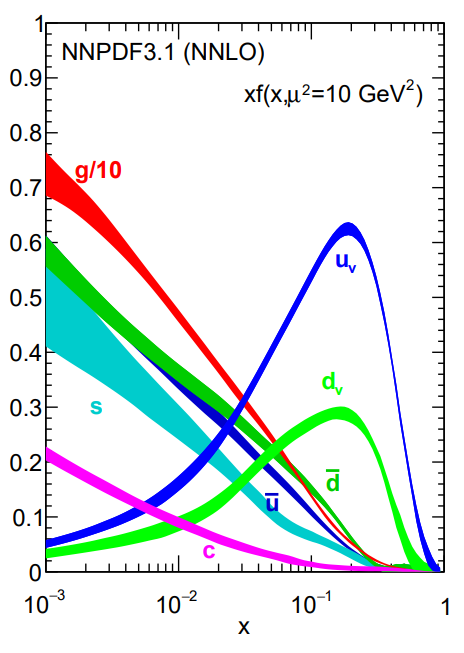
\includegraphics[width=0.7\linewidth]{NNPDF10.PNG}
	\end{minipage}
	\hfill
	\begin{minipage}[t]{0.48\linewidth}
		\centering
		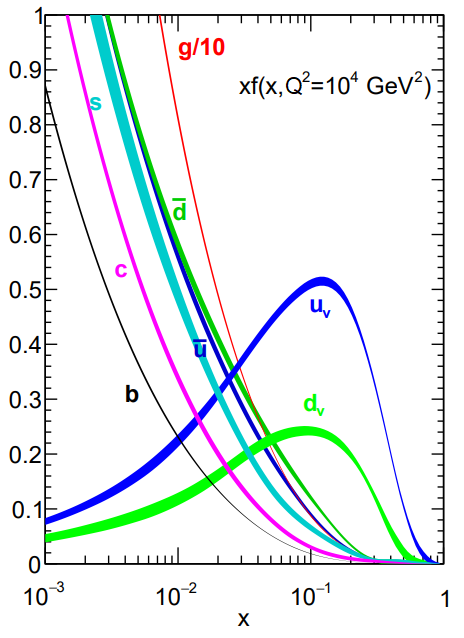
\includegraphics[width=0.7\linewidth]{NNPDF10000.PNG}
	\end{minipage}
	\vspace{-0.3cm}
	\captionof{figure}{ \label{fig:PDFs}
		NNPDF grupės pateikiamos protono partonų pasiskirstymo funkcijos esant skirtingoms susidūrimų energijoms \cite{NNPDF}.
		Kairėje -- $Q^{2}=10 \; \mathrm{GeV}^{2}$, dešinėje -- $Q^{2}=10000 \; \mathrm{GeV}^{2}$.
		Ant horizontalios ašies vaizduojama protono impulso dalis $x$, o ant vertikalios -- tikimybės tankio $f(x,\, Q^2)$
		ir $x$ sandauga.
	}
\end{centering}


\subsubsection{Drell-Yan procesas}

Drell-Yan procesas -- tai toks procesas, kai protonų susidūrimo metu anihiliavus kvarkui ir antikvarkui
sukuriama leptono ir antileptono pora.
Šis procesas vyksta apsikeičiant $Z$ bozonu arba
virtualiu fotonu per s-kanalą (\ref{fig:DYfeyn})

\begin{equation*}
	q\bar{q} \rightarrow Z/ \gamma^{*} \rightarrow l^{+}l^{-} \; .
\end{equation*}
Toliau bus žymima $\DY \! \rightarrow \! l^{+}l^{-}$.
Skirtingos Drell-Yan proceso galutinės būsenos, priklausomai nuo to, kokios rūšies leptonai susidaro, yra
vadinamos kanalais: elektronų kanalas, miuonų kanalas, taonų kanalas.

Drell-Yan procesas tapo svarbiu tyrimo objektu nuo pat pirmojo jo aprašymo $1970$-aisiais
metais, kai S.\ D.\ Drell ir T.\ M.\ Yan bandė apibūdinti leptonų ir antileptonų porų susidarymą
hadronų susidūrimų metu \cite{DYoriginal}.

Šiais laikais, naudojantis pertubacine kvantine chromodinamika, Drell-Yan procesas teoretikų
gali būti aprašomas trečios eilės perturbacijų tikslumu (angl.\ \textit{next-to-next-to-leading
order} -- NNLO).
Tikslūs eksperimentiniai Drell-Yan proceso diferencialinio skerspjūvio matavimai naudojami
ne tik partonų pasiskirstymo funkcijoms tikslinti, bet taip pat ir perturbacinės kvantinės
chromodinamikos bei elektrosilpnosios sąveikos teorijoms tikrinti.
Be to, šis procesas yra vienu iš pagrindinių triukšmo procesų įvairiuose kituose tyrimuose,
todėl tikslūs Drell-Yan proceso matavimai įvairiapusiškai prisideda prie kitų didelių energijų
fizikos tyrimų rezultatų kokybės.

\begin{figure}[H]
\centering
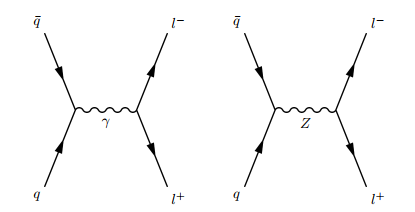
\includegraphics[scale=0.75]{DYprocess.PNG}
\caption{Drell-Yan proceso Feynman'o diagramos.}
\label{fig:DYfeyn}
\end{figure}


\subsubsection{Reakcijos skerspjūvis}

Drell-Yan proceso ir kitų didelių energijų fizikos procesų tikėtinumo aprašymui naudojamas
reakcijos skerspjūvis, kuris dažniausiai matuojamas barnais ($1$ b $= 10^{-28}$ m$^{2}$).
Skerspjūvio vertė nepriklauso nuo greitintuvuose lekiančių dalelių spindulių matmenų bei tankių,
Tad galima nesunkiai lyginti tam tikrų įvykių reakcijos skerspjūvius, išmatuotus skirtinguose dalelių
greitintuvuose.

Norint labiau pasigilinti į tam tikras tiriamo proceso charakteristikas būna naudojami diferencialiniai
reakcijos skerspjūviai $\mathrm{d}\sigma/\mathrm{d}\xi$ -- tai funkcijos, apibūdinančios tikėtinumą, kad mus
dominantis procesas ne tik įvyks, bet dar ir mūsų pasirinktas, rezultatą apibūdinantis tolydus
dydis $\xi$ pateks į tam tikrą intervalą $\mathrm{d}\xi$.

Drell-Yan proceso tyrime matuojami diferencialiniai reakcijos skerspjūviai, priklausantys nuo
leptonų poros invariantinės masės, skersinio impulso, spartos ir skilimo kampo:
$\mathrm{d}\sigma / \mathrm{d}m$, $\mathrm{d}\sigma / \mathrm{d}p_{\mathrm{T}}$, arba
$\mathrm{d}\sigma / \mathrm{d}y$, $\mathrm{d}\sigma / \mathrm{d}\Omega(\cos\theta, \phi)$.
Taip pat galimi ir keliamačio diferencialinio skerspjūvio matavimai, priklausantys nuo kelių
(arba visų) iš išvardintų dydžių.
Ganėtinai išsiskiriančią charakteristiką turi nuo leptonų poros invariantinės masės priklausantis
diferencialinis skerspjūvis, dar vadinamas invariantinės masės spektru -- jis yra rezonansinė
kreivė -- turi maksimumus ties fotono mase ($0$ GeV) ir $Z$ bozono mase (apie $91.2$ GeV).
Nuo masės priklausančio diferencialinio skerspjūvio pavyzdys pateikiamas \ref{fig:DYeeCS} paveiksle.


\subsubsection*{Invariantinė masė} 

Invariantinė masė -- tai masė, kuri nepriklauso nuo atskaitos sistemos.
Skaičiuojant vienos dalelės invariantinę masę, ji sutampa su jos rimties mase:

\begin{equation}
	m_{0}^{2}c^{4} = E^{2} - | \vec{p}\, |^{2}c^{2} \; .
	\label{eq:invm}
\end{equation}
čia $m_{0}$ -- dalelės invariantinė masė, $E$ -- pinoji dalelės energija, $\vec{p}$ -- dalelės impulso
vektorius, $c$ -- šviesos greitis.

Taip pat galima apskaičiuoti ir kelių dalelių sistemos invariantinę masę.
Pastaroji nėra lygi dviejų dalelių rimties masių sumai.
Jeigu dalelės, kurių sistemai skaičiuojame invariantinę masę, yra kažkokios kitos pradinės dalelės
skilimo produktai, tai gauta vertė bus lygi skilusios pradinės dalelės rimties masei.
Kelių dalelių sistemos invariantinė masė skaičiuojama taip:
\begin{equation}
	m_{\mathrm{sistemos}}^{2}c^{4} = \left( \sum_{n=1}^{N} E_{n} \right)^{2} -
	\left| \sum_{m=1}^{N} \vec{p}_{m} \right|^{2}c^{2} \; .
	\label{eq:minvm}
\end{equation}
Dviejų dalelių atveju:
\begin{equation}
	m_{12}^{2}c^{4} = ( E_{1} + E_{2} )^{2} - | \vec{p}_{1} + \vec{p}_{2} |^{2}c^{2} \; .
	\label{eq:tinvm}
\end{equation}
Būtent taip yra skaičiuojama Drell-Yan proceso metu susidariusių dviejų leptonų invariantinė masė.

\begin{centering}
\begin{figure}[H]
\centering
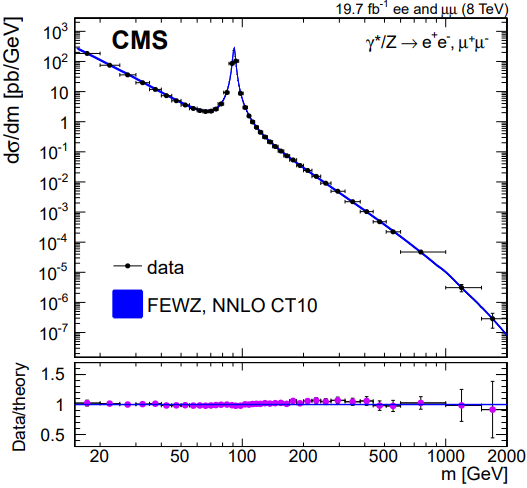
\includegraphics[scale=0.6]{DYeeCS.PNG}
\vspace{-0.2cm}
\caption{\label{fig:DYeeCS}
Nuo leptonų poros invariantinės masės priklausantis Drell-Yan proceso diferencialinis reakcijos skerspjūvis.
Protonų susidūrimo energija -- $8$ TeV.
Mėlyna ištisinė linija grafike žymi teorinį įvertį, o taškai su neapibrėžtumus žyminčiais brūkšniais --
eksperimentinį rezultatą \cite{DYpic}.
% GALIMA ĮDĖTI ŠITĄ https://cds.cern.ch/record/2648776/files/SMP-17-001-paper-v14.pdf
% 13 TEV, BET ČIA DRAFT VERSIJA
}
\end{figure}
\end{centering}


\subsubsection*{Sparta ir pseudosparta}

Sparta (angl.\ \textit{rapidity}) -- tai dalelių fizikoje naudojamas dydis, kuris yra patogus tuo,
kad dviejų dalelių spartų skirtumas nepakinta perėjus į bet kokią kitą išilgai cilindrinių koordinačių
$z$ ašies judančią sistemą (yra invariantas).
Sparta yra žymima raide $y$ ir apibrėžiama tokia formule:

\begin{equation}
	y = \frac{1}{2} \ln{ \left( \frac{E+p_{z}c}{E-p_{z}c} \right) } \; \mathrm{,}
	\label{eq:rapidity}
\end{equation}
čia $E$ -- dalelės energija, $p_{z}$ -- dalelės impulso projekcija į $z$ ašį, $c$ -- šviesos greitis.
Kai dalelė juda reliatyvistiniais greičiais,jos pilnutinę energiją galima aproksimuoti kinetine energija:

\begin{equation}
	E^2 = m^2c^4 + |\vec{p}|^2c^2 \approx |\vec{p}|^2c^2 \; .
	\label{eq:relEnergy}
\end{equation}
Panaudojus tokią aproksimaciją, dalelės spartą galima apytiksliai apskaičiuoti taip:

\begin{equation}
	y_{v\rightarrow c} = -\ln \left( \tan \frac{\theta}{2} \right) = \eta \; \mathrm{,}
	\label{eq:pseudorapidity}
\end{equation}
Tokia spartos aproksimacija vadinama pseudosparta ir žymima raide $\eta$.
Čia $\theta$ -- kampas, kurį sudaro dalelės impulso vektorius su $z$ ašimi ($0\leqslant \theta \leqslant \ang{180}$).
Šiuolaikiniuose dalelių greitintuvuose, kai dalelės juda beveik šviesos greičiu ir kai tiksliai
išmatuoti dalelės impulsą arba energiją išilgai $z$ ašies yra neįmanoma, vietoje spartos
yra naudojama pseudosparta.
Tiek sparta, tiek pseudosparta esant $\theta=\ang{90}$ yra lygios nuliui, o esant $\theta=\ang{0}$ --
begalybei (arba minus begalybei, kai $\theta=\ang{180}$).


\subsubsection*{Skersinis impulsas ir skersinė energija}

Kadangi, dalelių detektorius yra cilindriškai išdėstytas aplink protonų spindulį, dalelės impulso
projekcijos į cilindrinės koordinačių sistemos $z$ ašį nustatyti yra neįmanoma.
Dėl šios priežasties šiuolaikiniuose dalelių detektoriuose, tokiuose kaip CERN CMS yra matuojama tik
statmena $z$ ašiai dalelės impulso dedamoji arba šio judėjimo nulemtos kinetinės energijos dedamoji.
Šie dydžiai yra vadinami skersiniu impulsu $\pT$ (angl.\ \textit{transverse momentum}) ir
skersine energija $\ET$ (angl.\ \textit{transverse energy}).
Išmatavus skersinį impulsą kartu su dalelės sparta $\eta$ ir azimutiniu kampu $\phi$ bei žinant dalelės
masę galima pilnai aprašyti dalelės judėjimą taip pat, kaip ir žinant dalelės pilnutinę energiją bei
impulso dekartines dedamąsias.

Taip pat galima pastebėti, kad žinant dalelės skersinį impulsą ir pseudospartą, galima apskaičiuoti ir
jos pilnutinio impulso vertę:

\begin{equation}
	|\vec p|=p_{\mathrm{T}}\cosh\eta \; .
	\label{eq:pmodpt}
\end{equation}


\subsubsection*{Šviesis}

Šviesis -- tai dydis, apibūdinantis skaičių dalelių, per laiko vienetą pralėkusių per mus dominantį plotą.
Šviesis žymimas raide $\mathcal{L}$ (angl.\ \textit{luminosity}).

Norint apibūdinti dalelių greitintuvuose vykstančių susidūrimų skaičių, naudojamas šviesio
laikinis integralas -- integruotasis šviesis:

\begin{equation}
	\Lumi=\int_{t_1}^{t_2} \mathcal{L}\mathrm{d}t =
	\int_{t_1}^{t_2} \frac{1}{\sigma}\frac{\mathrm{d}N}{\mathrm{d}t} \mathrm{d}t \; .
\label{eq:lumiInt}
\end{equation}

Iš \eqref{eq:lumiInt} išraiškos galima matyti, kad integruotasis šviesis turi atvirkštinio ploto
matavimo vienetus.
Eksperimentinėje didelių energijų fizikoje šis dydis matuojamas atvirkštiniais barnais -- $b^{-1}$.
Sudauginus integruotą šviesį su tam tikro įvykio skerspjūviu galime gauti, kiek kartų tas įvykis
turėtų įvykti -- taip pat, kaip ir sudauginus įvykio tikimybę su bandymų skaičiumi:

\begin{equation}
	N=\sigma\Lumi \; .
\label{eq:evno}
\end{equation}

Eksperimentinėje didelių energijų fizikoje labai svarbu tiksliai apskaičiuoti integruotą šviesį,
nes jis susieja teorinį įvykio aprašymą (skerspjūvį) su tuo, kas fiksuojama eksperimente (įvykių skaičius).


\subsection{Drell-Yan proceso eksperimentinis tyrimas}

\subsubsection{Signalas ir triukšmas}\label{sec:SignalBkg}

CERN Didžiajame hadronų greitintuve vykstančių $13$ TeV energijos protonų susidūrimų metu gali
būti sukurtos labai masyvios ir labai trumpai gyvuojančios dalelės.
Tokios dalelės skyla nespėjusios pasiekti detektoriaus, todėl fiksuojami yra tik šių dalelių
skilimo produktai -- ilgiau gyvuojančios ir mums gerai pažįstamos dalelės (pavyzdžiui,
elektronai, fotonai, įvairių rūšių hadronai, miuonai).
Detektoriuje užfiksuojamos dalelės su savo parametrais yra vadinamos įvykio galutine būsena
(angl.\ \textit{final state}).
Vykdant tokio tipo eksperimentą yra sunku vienareikšmiškai nuspręsti, kad detektoriuje užfiksuotos
dalelės yra konkrečios dalelės skilimo produktai.
Pavyzdžiui, tiriant Drell-Yan procesą galima ieškoti įvykio, kurio metu susidarė du elektronai.
Čia turima omenyje, kad užfiksuota elektrono-pozitrono pora.
Trumpumo sumetimais didelių energijų fizikoje dalelės ir antidalelės dažnai vadinamos tuo
pačiu (dalelės) vardu.
Tačiau pamatę detektoriaus užfiksuotus du elektronus
negalime teigti, kad matome būtent Drell-Yan proceso įvykį.
Labai panašiai gali atrodyti ir, pavyzdžiui, protonų susidūrimo metu sukurtos viršūninio ir
antiviršūninio kvarko poros leptoninio skilimo produktai.
Tokiu atveju sakome, kad elektronų pora, susidariusi Drell-Yan proceso metu, yra signalas, o
pora, susidariusi iš viršūninių kvarkų poros -- triukšmas (angl.\ \textit{background}), į
kurio egzistavimą reikia atsižvelgti.

Taip pat protonų susidūrimo metu dėl stipriosios sąveikos efektų gali susidaryti dalelių
srautai, vadinami čiurkšlėmis (angl.\ \textit{jets}).
Pasitaiko atvejų, kai detektoriuje užfiksuotos \ltq{greitosios} čiurkšlės yra neteisingai atpažįstamos kaip
kitos dalelės (pavyzdžiui, elektronas).
Taigi, įvykiai su čiurkšlėmis taip pat sukuria triukšmą.

Nors pavyzdyje buvo kalbama tik apie elektronų poros galutinę būseną (sutrumpintai bus
žymima $ee$), šiame darbe dar buvo tiriama ir miuonų poros galutinė būsena (sutrumpintai $\mumu$).	 
Dviejų taonų galutinė būsena nebuvo tiriama dėl gan smarkiai besiskiriančios tyrimo metodikos
(taonai skyla į kitas daleles nepasiekę detektoriaus). Įdomu tai, kad šiuo atveju tiek tiriant
miuonų, tiek elektronų galutines būsenas, Drell-Yan proceso taonų kanalas
yra triukšmas. Kiti pagrindiniai triukšmai yra šie: viršūninių kvarkų (angl.\ \textit{top quark})
poros įvykiai (sutrumpintai bus žymima $t\bar{t}\,$), dviejų bozonų įvykiai ($WW$, $WZ$ ir $ZZ$),
vieno viršūninio kvarko ir $W$ bozono įvykiai ($tW$), $W$ bozono ir čiurkšlės įvykiai ($\WJets$),
bei stipriosios sąveikos nulemti keletos čiurkšlių įvykiai (sutrumpintai vadinami $\QCD$).

Kaip buvo rašoma ankstesniame skyrelyje, norint palyginti eksperimento metu užfiksuotą
statistiką su teoriškai numatomu rezultatu, svarbu įvertinti, kaip smarkiai užregistruoti
pasiskirstymai yra užteršti triukšmų.
Kadangi didelių energijų fizikos eksperimentinių duomenų analizė prasideda nuo tam tikrus
reikalavimus atitinkančių įvykių skaičiavimo, yra taikomi įvairūs metodai
tokius reikalavimus atitinkančių įvykių skaičiaus numatymui.
Tada galima lyginti, ar išmatuotas rezultatas atitinka numatytąjį.
Didelių energijų fizikoje pagrindinai yra naudojamos dvi metodikos: Monte Carlo (MC) modeliavimas
ir matavimu grįsti metodai.

\subsubsection*{Monte Carlo modeliavimas}

Norint gauti teorinį eksperimento rezultatų įvertį galima kiek norima kartų atlikti virtualų
eksperimentą.
Kad tokį eksperimentą būtų galima atlikti, reikia turėti teoriją, kuri numato tam tikro mus
dominančio įvykio tikimybės pasiskirstymą, bei turėti atsitiktinių skaičių generatorių.
Generuojant atsitiktinius skaičius pagal tam tikrą tikimybės pasiskirstymą galima sumodeliuoti
įvykius, su kuriais darant tas pačias analizės procedūras, kaip ir su eksperimento metu
užregistruotais įvykiais, galime gauti rezultatą, palyginamą su realybėje išmatuotu
rezultatu -- teorinį įvykių skaičiaus įvertį.

Aišku, realybėje didelių energijų protonų sklaidos eksperimentų modeliavimas nėra toks
tiesmukas.
Įprastiniu atveju, Didžiajame hadronų greitintuve vykstančių protonų susidūrimo įvykių
modeliavimas vykdomas keliais etapais.
Pirmiausia sumodeliuojamas pats protonų susidūrimas -- sugeneruoti atsitiktiniai skaičiai
transformuojami į įvykio rezultatą -- kokios dalelės susidarė bei kokie jų parametrai
(koordinatė, greitis ir pan.).
Po to modeliuojamas susidariusių dalelių sklidimas ir sąveika su medžiaga -- dalelių
detektoriaus komponentais.
Taip sumodeliuojama, ką galėjo užregistruoti detektorius įvykus būtent tokiam įvykiui.
Galiausiai gaunamas rezultatas, kuris savo išvaizda nesiskiria nuo tikro eksperimento metu
užregistruotų duomenų.
Tokiu būdų eksperimentatoriams yra labai patogu lyginti realiai gautą rezultatą su teoriniu.

CERN Kompaktiškojo miuonų solenoido (angl.\ \textit{Compact Muon Solenoid} -- CMS) eksperimente
įvykių modeliavimui dažniausiai naudojami šie programiniai paketai:
\begin{itemize}
	\item \textsc{Pythia8} -- tai C++ kalba parašytas programinis paketas, skirtas modeliuoti
	didelių energijų dalelių susidūrimus.
	\textsc{Pythia} paskirtis labai plati -- ji tinkama modeliuoti praktiškai bet kokiems žinomiems protonų
	susidūrimo metu vykstantiems procesams, joje yra įrašyta daug skirtingų teorinių modelių,
	partonų pasiskirstymo funkcijų.
	Su \textsc{Pythia} įvykius galima modeliuoti tik pirmos eilės (angl.\ \textit{leading order} -- LO)
	perturbacijų tikslumu \cite{pythia82}.
	
	\item \ttt{aMC@NLO} -- tai plačios paskirties Python pagrindo programinės įrangos rinkinys,
	leidžiantis skaičiuoti reakcijų skerspjūvius, modeliuoti didelių energijų dalelių susidūrimus
	bei atlikti jų analizę.
	Naudojantis šiuo programiniu paketu galima modeliuoti įvykius iki antros eilės perturbacijų
	(angl.\ \textit{next-to-leading order} -- NLO) tikslumo \cite{amcatnlo}.
	
	\item FEWZ -- tai Fortran pagrindo programinis paketas, skirtas modeliuoti  $W$ ir $Z$
	bozonų susidarymą hadronų susidūrimo metu, taip pat šių bozonų skilimus į leptonus ir pan.
	FEWZ taip pat palaiko nemažai skirtingų partonų pasiskirstymo funkcijų bei modeliuoja įvykius
	trečios eilės perturbacijų (angl.\ \textit{next-to-next-to-leading order} -- NNLO) tikslumu \cite{fewz}.
	
	\item \textsc{Geant4} -- tai C++ pagrintdo programinis paketas, skirtas modeliuoti dalelių sąveiką
	su medžiaga.
	\textsc{Geant4} yra tinkama modeliuoti praktiškai bet kokių stabilių dalelių sąveikai su medžiaga
	bei pataikymams į skirtingus detektoriaus komponentus \cite{geant4}.
	Kompaktiškojo miuonų solenoido eksperimente šis programinis paketas naudojamas viso CMS detektoriaus
	atsako į konkretų (jau sumodeliuotą naudojantis kita programine įranga) protonų susidūrimo įvykį
	modeliavimui.
	
	\item CMSSW (\textit{CMS SoftWare}) -- tai CERN CMS eksperimente visuotinai naudojamas programinės
	įrangos rinkinys, skirtas ne tik įvykių modeliavimo, bet taip pat ir  visiems reikiamiems duomenų
	gavimo, apdorojimo ir analizės darbams atlikti.
	CMSSW išnaudoja bendrą CMS duomenų formatą -- įvykių duomenų modelį (angl.\ \textit{Event Data Model}
	-- EDM, kuris tinkamas skirtingiems duomenų apdorojimo lygmenims bei analizės etapams.
	Joje yra tiek protonų susidūrimui, tiek detektoriaus atsakui modeliuoti skirti programiniai paketai
	(tokie, kaip jau minėti \textsc{Pythia8} ir \textsc{Geant4})
\end{itemize}

Modeliuotas įvykių skaičiaus įvertis dažniausiai laikomas nepakankamai tiksliu dėl neapibrėžtumų,
kuriuos įneša nepakankamai tikslios žinios apie atskirų triukšmo procesų įvykių tikėtinumus,
neidealus detektoriaus atsako modeliavimas ir pan.
Šių problemų gali būti išvengiama triukšmo įvykių skaičiaus įvertinimui naudojant matavimu
grįstus metodus.

\subsubsection*{Matavimu grįsti metodai}

Matavimu grįsti triukšmo įvykių skaičiaus įvertinimo metodai apima ir matavimą, ir modeliavimą.
Su skirtingos specifikos procesais siejamų įvykių skaičiui įvertinti naudojami skirtingi
matavimu grįsti metodai, tačiau jie visi remiasi labai panašia ideologija.
Pagrindinis matavimu grįstų įvykių skaičiaus įvertinimo metodų principas remiasi signalo ir
kontrolinės sričių apibrėžimais.
Signalo sritis (angl. \textit{signal region}) -- tai fazinės erdvės dalis, apribota tokiais
parametrais, kad į ją patektų kuo didesnė dalis signalo įvykių (tačiau neišvengiamai patenka
ir kažkiek triukšmo įvykių).
Kontrolinė sritis (angl. \textit{control region}) -- tai fazinės erdvės dalis, apribota
tokiais parametrais, kad į ją patektų kuo daugiau triukšmo įvykių ir, idealiu atveju, signalo
įvykių nepatektų išvis.
Kiekvienas matavimu grįstas metodas turi savo specifinę operaciją, kuria triukšmo įvykių skaičius,
išmatuotas kontrolinėje srityje, yra transformuojamas į triukšmo įvykių skaičių, patenkantį į
signalo sritį:

\begin{equation}
	N_{\mathrm{Bkg}}^{\mathrm{Signal}} = f( N_{\mathrm{Bkg}}^{\mathrm{Control}} )
	\label{eq:data-driven}
\end{equation}

Vieni iš populiariausių matavimu grįstų metodu yra klaidingo atpažinimo (angl.
\textit{fake rate} -- FR) ir ABCD metodai.
Jie naudojami įvertinti skaičiui tokių triukšmo įvykių, kurių metu susidarė čiurkšlės.
Tokių triukšmo įvykių, kurių metu gali susidaryti keli vienodų arba skirtingų
rūšių leptonai, skaičiui įvertinti naudojamas $\emu$ metodas, kuris ir buvo naudojamas šiame
darbe.

\paragraph{$e\mu$ metodas\\}

$\emu$ metodas -- tai matavimu grįstas triukšmo įvykių skaičiaus įvertinimo metodas, kuris
naudojamas dviejų vienodų leptonų (elektronų arba miuonų) galutinės būsenos triukšmams
įvertinti, pasinaudojant įvykių, kuriuose buvo užfiksuoti skirtingi leptonai (elektronas
ir miuonas), duomenimis.
Šis metodas tinkamas įvertinti tokiems triukšmams, kurie siejami su dviejų nestabilių
dalelių, kurios turi galimybę nepriklausomai viena nuo kitos skilti į leptonus, susidarymu.
Tokie triukšmo procesai yra: $\WW$, $\WZ$, $\ZZ$, $tW$, $\tbarW$, $\ttbar$, $\DYtau$.
Galima nesunkiai matyti, kad visuose šiuose procesuose figūruoja dvi sunkios dalelės, kurios
gali skilti leptoniškai.

Kaip pavyzdį $\emu$ metodo veikimui paaiškinti galime paimti $WW$ procesą.
Jeigu nagrinėjame tik $W$ bozono skilimus į elektroną arba miuoną (kartu su atitinkamais
neutrinais), tai turėdami įvykį, kurio metu susidaro du $W$ bozonai, galime turėti
keturias skirtingas galutines būsenas: $WW \! \rightarrow \! e^+e^-$,
$WW \! \rightarrow \! e^+\mu^-$, $WW \! \rightarrow \! \mu^+e^-$ ir
$WW \! \rightarrow \! \mu^+\mu^-$.
Čia dešinėje rodyklės pusėje nerašėme atitinkamų neutrinų, nes $\emu$ metodo skaičiavimuose
jie nedalyvauja.
Pasinaudodami Monte Carlo modeliavimu galime įsivertinti $ee$ ir $\emu$ įvykių skaičiaus
santykį $N_{ee}^{\mathrm{MC}} / N_{\emu}^{\mathrm{MC}}$, nekreipdami dėmesio į elektrono
ir miuono elektrinius krūvius, tik reikalaudami, kad jie būtų skirtingi.
Idealiu atveju šis santykis turėtų būti apytiksliai lygus $1:2$, nes tiek elektrono, tiek
miuono masės santykis su motininės dalelės mase yra labai mažas.
Tai reiškia, kad nestabili dalelė gali skilti į miuoną arba elektroną su apytiksliai
vienoda tikimybe.
Padarius prielaidą, kad šis santykis turėtų būti vienodas tiek eksperimentiniuose, tiek
modeliuotuose duomenyse, galime įvertinti (angl.\ \textit{estimate}), koks turėtų būti su
anksčiau minėtais procesais susijusių triukšmo įvykių skaičius $ee$ duomenyse:

\begin{equation}
	N_{ee}^{t\bar{t} , \; \mathrm{Est}} =
	\frac{ N_{ee}^{t\bar{t} , \; \mathrm{MC}} }{ N_{e\mu}^{t\bar{t} , \; \mathrm{MC}} }
	\cdot N_{e\mu}^{t\bar{t} , \; \mathrm{Data}} \; .
	\label{eq:emuMethod}
\end{equation}

Vis dėlto, ši išraiška yra idealizuota, nes realybėje neįmanoma iš eksperimentinių duomenų
vienareikšmiškai išskirti, kurie įvykiai yra sietini su konkrečiu procesu (šiuo atveju --
$\ttbar$), todėl formulę reikia taikyti visiems $\emu$ procesams iškart:

\begin{equation}
	N_{ee}^{\mathrm{Įv.}} =
	\frac{ N_{ee}^{\mathrm{MC}} }{ N_{\emu}^{\mathrm{MC}} }
	\cdot N_{\emu}^{\mathrm{Data}} \; .
	\label{eq:emuReal}
\end{equation}

Prisiminus \eqref{eq:data-driven} išraišką ir palyginę ją su \eqref{eq:emuReal} galime
sakyti, kad $N_{t\bar{t}}^{ee , \; \mathrm{Data}}$ yra signalo sritis, o
$N_{t\bar{t}}^{e\mu , \; \mathrm{Data}}$ yra kontrolinė sritis. Joje yra vien tik triukšmo
įvykiai.
Triukšmo įvykių skaičiaus signalo srityje įvertį gauname su triukšmo įvykių skaičiumi
kontrolinėje srityje atlikę paprastą matematinę operaciją -- padauginę jį iš modeliuotų
$ee$ ir $\emu$ įvykių skaičiaus santykio.


\subsubsection{Modeliuotų įvykių skaičiaus normavimas}\label{sec:MCweight}

Jeigu kokio nors mus dominančio proceso tikėtinumą aprašo jo skerspjūvis $\sigma$, tai atlikus
$\Lumi$ integruotą šviesį atitinkančių protonų susidūrimų mus dominanti įvykis teoriškai turėtų
įvykti $N_{0}$ kartų. Pagal \eqref{eq:evno} formulę:
\begin{equation}
	\sigma \Lumi=N_{0} \; .
	\label{eq:ilumi}
\end{equation}

Išmatuotos mus dominančių įvykių statistikos palyginimui su teorija galime sumodeliuoti tiek mus
dominantį procesą atitinkančių įvykių, kiek jų norime, arba kiek leidžia turimi resursai.
Bendru atveju sumodeliuotų įvykių skaičius $N$ nesutampa su eksperimente užregistruotų įvykių
skaičiumi $N_0$, todėl modeliuotus įvykius reikia sunormuoti, kad atitiktų eksperimentinį
integruotą šviesį.
Tai yra daroma kiekvienam modeliuotam įvykiui priskiriant po tam tikrą svorį $\omega$:

\begin{equation}
	\sum_{i=1}^{N} \omega_{i}=N_{0} \; .
	\label{eq:wsum}
\end{equation}

Paprasčiausiu atveju visiems modeliuotiems įvykiams, kurie yra siejami su tuo pačiu procesu,
galima priskirti vienodus svorius.
Tokiu atveju \eqref{eq:wsum} išraiškoje esanti suma tampa lygi $N\omega$, o kiekvieno įvykio
svoris gali būti apskaičiuojamas taip:

\begin{equation}
	\omega = \frac{ N_{0} }{ N } = \frac{ \sigma \Lumi }{N} \; .
	\label{eq:weight}
\end{equation}

Kai naudojama programinė įranga geba modeliuoti įvykius aukštesniu, nei pirmos eilės
perturbacijų tikslumu, neretai skirtingiems įvykiams pats įvykių generatorius jau iškart
gali priskirti skirtingus svorius.
Tokiu atveju modeliuotų įvykių svorių sumos išraiškos negalima supaprastinti ir svorinis
daugiklis, priskiriamas kiekvienam įvykiui apskaičiuojamas taip:

\begin{equation}
	\omega_{i}^{\mathrm{Piln.}} = \omega_{i} \frac{ \sigma\Lumi }{ \sum_{i=j}^{N}\omega_{j} } \; .
	\label{eq:NLOweight}
\end{equation}

\subsubsection{Didysis hadronų greitintuvas ir Kompaktiškasis miuonų solenoidas}

Šveicarijos - Prancūzijos pasienyje esantis Europos branduolinių tyrimų organizacijai CERN
priklausantis Didysis hadronų priešpriešinių srautų greitintuvas yra didžiausias ir galingiausias
dalelių greitintuvas pasaulyje.
Maždaug $27$ km perimetro žiedinis greitintuvas slepiasi apytiksliai $100$ m gylyje po žeme.
Nors didžiajame hadronų greitintuve galima vykdyti įvairių hadroninių dalelių (pavyzdžiui, švino
branduolių) susidūrimus, dažniausiai ten vykdomi ir daugiausiai tiriami yra protonų susidūrimai.
Dalelės, prieš patekdamos į šį greitintuvą praeina kelias greitinimo pakopas kituose mažesniuose
greitintuvuose, kurie anksčiau buvo naudojami vykdyti dalelių susidūrimams \cite{accelerators}.
Nuo $2015$ metų Didžiajame hadronų greitintuve vykstančių protonų susidūrimų energija sieka net $13$ TeV.
Įprastai jie vyksta kas $25$ ns keliuose skirtinguose žiedo taškuose, aplink kuriuose yra išdėstyti dalelių
detektoriai, priklausantys skirtingų eksperimentų grupėms.
Dvi didžiausios ir geriausiai žinomos eksperimentinės grupės yra CMS ir ATLAS.

Kompaktiškasis miuonų solenoidas (angl.\ \textit{Compact Muon Solenoid} -- CMS) yra plačios paskirties
detektorius, sukurtas įvairių skirtingų dalelių detektavimui.
Dėl šios priežasties CMS eksperimento mokslininkai gali vykdyti labai skirtingų tematikų tyrimus,
pavyzdžiui, tikslinti ir tikrinti Standartinį modelį, ieškoti naujų dalelių arba net papildomų
dimensijų ar tamsiosios medžiagos \cite{aboutCMS}.

CMS yra cilindrinės geometrijos detektorius, jo aukštis ir plotis -- apytiksliai po $15$ m, o ilgis --
apie $21$ m.
Detektorius vadinamas kompaktiškuoju todėl, kad kaip tokių matmenų jis yra labai masyvus.
Jo masė -- apytiksliai $14000$ tonų.
Detektorius susideda iš daug sluoksnių ir segmentų, kurie skirti detektuoti skirtingų rūšių dalelėms.
CMS \ltq{širdis} -- didžiausias pasaulyje solenoidinis elektromagnetas.
Tai iki superlaidumo temperatūros atšaldoma ritė, kuria darbo metu teka $19.1$ kA stiprio elektros srovė,
ir kurios viduje sukuriamas iki $4$ T siekiantis magnetinis laukas.

CMS detektoriaus segmentus galima pamatyti \ref{fig:CMSslice} paveiksle.
Kiekvienas detektoriaus segmentas turi cilindrinę ir antgalių dalis, kurios yra sluoksniškai išdėstytos
einant tolyn nuo protonų susidūrimo vietos.
Kiekvienas subdetektorių sluosknis yra skirtingas ir turi savo paskirtį \cite{CMSexperiment}.

Arčiausiai aplink protonų spindulį yra išdėstytas trekų detektorius (angl.\ \textit{silicon tracker}),
pagamintas iš silicio pikselių ir juostelių.
Į trekų detektorių pataikiusios elektringos dalelės išlaisvina krūvininkus taip sugeneruodamos elektrinį
signalą.
Iš užfiksuoto signalo keliose skirtingose trekų detektoriaus dalyse galima nustatyti, kokia kryptimi
nulėkė protonų susidūrimo metu sukurtos elektringosios dalelės.

Tolimesnis sluoksnis einant nuo protonų susidūrimo taško yra elektromagnetinis kalorimetras (angl.\
\textit{Electromagnetic Calorimeter} -- ECAL).
Šio subdetektoriaus paskirtis -- detektuoti elektronus ir fotonus.
Svarbiausia elektromagnetinio kalorimetro sudedamoji dalis -- scintiliatorius švino volframatas $\mathrm{PbWO}_{4}$,
kuris ima švytėti, kai į jį pataiko energingas elektronas arba fotonas \cite{ECALtrig}.
Šios dalelės dažniausiai čia praranda visą savo kinetinę energiją, kuriai sukelto švytėjimo intensyvumas
būna proporcingas.
Dėl šios priežasties elektromagnetiniu kalorimetru galima išmatuoti, su kokia energija dalelė atlėkė.
Elektroną nuo fotono galima atskirti pagal tai, ar galima susieti kalorimetre užfiksuotą signalą su trekų
detektoriuje užregistruotu treku.

Dar toliau nuo protonų spindulio yra išsidėstęs hadronų kalorimetras (angl.\ \textit{hadron calorimeter} -- HCAL).
Šio subdetektoriaus veikimo principas panašus į elektromagnetinio kalorimetro, tik šis skirtas detektuoti
hadronus bei išmatuoti jų energiją.
Tačiau yra ir didesnių skirtumų: čia naudojamas plastiko scintiliatorius, bei, kadangi hadronai yra gerokai
sunkesni ir skvarbesni, norint juos sustabdyti tarp scintiliatoriaus sluoksnių yra įterptos vario plokštės.
Taip pat šis subdetektorius yra gerokai storesnis už elektromagnetinį kalorimetrą.

Už hadronų kalorimetro yra jau minėtas superlaidus solenoidas.
Jo paskirtis -- iškreivinti krūvį turinčių dalelių trajektorijas.
Pagal tai, kuria kryptimi būna užsukta dalelės trajektorija, galima nustatyti, ar jos elektrinis krūvis buvo
teigiamas, ar neigiamas, bei nustačius, kokio tipo dalelė buvo užfiksuota, iš jos trajektorijos kreivumo
spindulio galima įvertinti dalelės impulsą.
Taip pat solenoidas veikia kaip papildomas stabdis skvarbiausiems hadronams.
Vis dėlto, norint užtikrinti, kad kuo mažiau hadronų pasiektų dar tolimesnius detektoriaus sluoksnius, už
solenoido yra sumontuotas papildomas hadronų kalorimetro sluoksnis, vadinamas išoriniu hadronų kalorimetru
(angl.\ \textit{HCAL outer}).

Išorinį hadronų kalorimetrą dar supa labai daug dėmesio sulaukianti detektoriaus dalis (tai ryškiai atsispindi
ir detektoriaus pavadinime) -- keliais sluoksniais išdėstyti miuonų detektoriai.
Nors miuonų detektorių sistemoje yra išnaudojami kelių skirtingų tipų detektoriai, jie visi yra priskiriami
tai pačiai dujinių detektorių kategorijai.
Miuonų detektoriai yra išrikiuoti toliausiai nuo protonų susidūrimo taško, nes jie yra apie $200$ kartų
sunkesni už elektronus, bei nesąveikauja stipriąja sąveika.
Dėl šios priežasties jie yra nesustabdomi nei elektromagnetiniame, nei hadronų kalorimetre.
Iš tiesų, jie nėra sustabdomi nei miuonų detektorių sistemoje -- dujiniai detektoriai tik užfiksuoja jų
trajektoriją.
Miuonų impulsas yra nustatomas iš jų trajektorijos kreivumo.
Kad tai būtų galima nustatyti kuo efektyviau, tarp miuonų detektorių yra sumontuotos geležinės magnetinio
lauko apgrąžos plokštės, kurios sustiprina už solenoido esantį magnetinį lauką ties miuonų detektoriais,
tuo pačiu neleisdamos jam tęstis toli už detektoriaus.
Taip pat šios plokštės užblokuoja kelią paskutinėms iki jų prasiskverbusioms dalelėms, kurios nėra miuonai
arba neutrinai.

\begin{figure}[H] \centering
	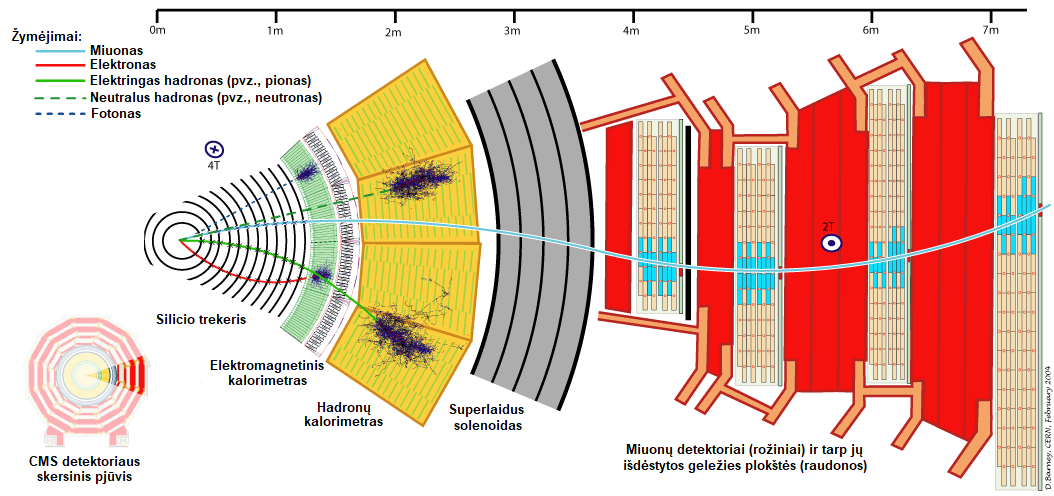
\includegraphics[width=0.95\textwidth]{CMSslice_LT.png}
	\caption{\label{fig:CMSslice}Skersinis CMS detektoriaus pjūvis \cite{CMSslice}.
	Išorinis hadronų kalorimetras nepavaizduotas. Skirtingos linijos žymi skirtingų dalelių, išlekiančių
	iš protonų susidūrimo vietos, trajektorijas.
	Trūki linija žymi elektriškai neutralios dalelės trajektoriją, kuri silicio trekų detektoriuje
	neužfiksuojama.}
\end{figure}

\subsubsection{Protonų susidūrimų atkūrimas}\label{sec:ppReco}

Po protonų susidūrimo susidariusios dalelės detektoriuose aptinkamos netiesiogiai, t.y., realiai  yra
užregistruojamas tik tam tikro pobūdžio signalas detektoriaus komponentuose, pagal kurį galima spręsti,
kad į jį pataikė tam tikra dalelė su tam tikra energija ir pan.
Tam, kad būtų galima gauti tam tikrą dalelę aprašančius fizikinius dydžius reikia gerai išmanyti, ką
ir kaip detektorius detektuoja.
O norint susidaryti pilną protonų susidūrimo vaizdą dar reikia apjungti visų detektoriaus komponentų
užregistruotą informaciją.
Šiam tikslui įgyvendinti yra naudojama sudėtingi programiniai algoritmai, iš kurių keletas bus trumpai
aprašyti.


\subsubsection*{Dalelių srautas}

Dalelių srautas (angl.\ \textit{particle flow} -- PF) -- tai įvykių atkūrimo algoritmas, savo tikslui pasiekti
naudojantis visų CMS subdetektorių užregistruotą informaciją.
Šis algoritmas naudoja iteracinę įvykių atkūrimo metodiką: pirmiausia naudodamasis smarkiai suvaržytais
atrankos kriterijais išrenka tas trajektorijas, dėl kurių yra \ltq{užtikrinčiausias}, bei apskaičiuoja
su jomis susijusius svarbius dydžius (pavyzdžiui, dalelės krūvį, skersinį impulsą, pseudospartą,
kokia dalelė apskritai susidarė ir pan.).
Po to šios atrinktos trajektorijos yra išimamos iš pilno duomenų bloko ir sekančioje iteracijoje iš
naujo bandoma išrinkti kitas trajektorijas šiek tiek sušvelninus atrankos kriterijus.
Taip trajektorijų atrinkimo procesas kartojamas kol panaudojama visa subdetektorių informacija.
Dalelių srauto įvykio atkūrimo rezultatas -- duomenys, kurie iš pažiūros atrodo taip pat kaip po
Monte Carlo protonų susidūrimo modeliavimo.
Vis dėlto, kadangi šis algoritmas negali visada dalelių atpažinti idealiai tiksliai, dažniausiai
atkurtos dalelės vadinamos dalelėmis kandidatėmis, o su tam tikru procesu siejami įvykiai --
įvykių kandidatais.
Drell-Yan proceso įvykio kandidato akurtas vaizdas pateikiamas \ref{fig:Event} paveiksle.

\begin{figure}[H]
	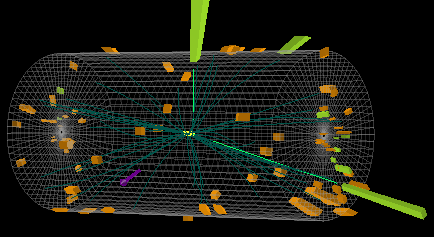
\includegraphics[width=0.8\textwidth]{Event.png}
	\caption{\label{fig:Event}
	Atkurto Drell-Yan proceso įvykio kandidato vaizdas, sugeneruotas su CMSSW pakete esančia programa FireWorks.
	Tamsiai žalsvos kreivės vaizduoja atkurtas mažos energijos dalelių (daugiausia pionų), o ryškiai žalios
	linijos -- didelės energijos elektronų trajektorijas.
	Ryškiai žalios ir oranžinės erdvinės figūros vaizduoja atitinkamai elektromagnetiniame ir hadronų kalorimetruose
	užregistruotus energijos kiekius.
	Šiame paveiksle galima matyti elektronų porą, kurios invariantinė masė yra apie $90$ GeV.
	}
\end{figure}

Dar dalelių srauto algoritmas apskaičiuoja nemažai daliai CMS vykdomų tyrimų svarbų dydį -- dalelės
kandidatės trajektorijos atskirumą (angl.\ \textit{isolation}).
Šis dydis apibrėžiamas kaip dalelių, patekusių į tam tikro pločio kūgį, nubrėžtą aplink tiriamosios
dalelės trajektoriją, skersinių impulsų suma.
Įprastai norima, kad ta suma būtų kuo mažesnė, arba, kitaip tariant, dalelės srautas kuo atskiresnis.
Tada norint būti labiau užtikrintam, kad, pavyzdžiui miuono kandidatas tikrai yra miuonas, galima
pritaikyti apribojimą, reikalaujanti, kad miuono kandidato trajektorijos atskirumas neviršytų tam tikro dydžio
(pavyzdžiui, $15\%$ paties miuono skersinio impulso vertės).

Norint patikslinti atskirumo skaičiavimo vertę neretai būna panaudojama pataisa, kuri atsižvelgia į
pašalinius protonų susidūrimus.
Kadangi protonų spinduliai detektoriuje susiduria kas $25$ ns (kol visos susidariusios dalelės
pasiekia detektorius gali įvykti dar keli nauji susidūrimai), bei vieno spindulių susidūrimo metu
dažniausiai susiduria daugiau negu viena protonų pora, tai svarbu yra atskirti, ar stebimos dalelės
yra susidariusios būtent mus dominančio protonų susidūrimo metu.
Dėl šios priežasties į atskirumo skaičiavimą būna įskaitomi dalelių, susidariusių pašalinių
protonų susidūrimo metu, skersiniai impulsai $p_{\mathrm{T}}^{\mathrm{PU}}$ (PU -- nuo angliško
termino \textit{pile-up}).
Santykinis leptonų kandidatų atskirumas apskaičiuojamas pagal tokią formulę:

\begin{equation}
	\label{eq:isolation}
	I^{\mathrm{rel.}}_{\mathrm{PF}} = \frac{1}{p_{\mathrm{T}}} 
	\left[ \sum_{\Delta R<0.3} p_{\mathrm{T}}^{\mathrm{hadron^{\pm}}} +
	\mathrm{max} \left( \sum_{\Delta R<0.3} p_{\mathrm{T}}^{\mathrm{hadron^0}} + 
	\sum_{\Delta R<0.3} p_{\mathrm{T}}^{\gamma} -
	\Delta \beta \sum_{\Delta R<0.3} p_{\mathrm{T}}^{\mathrm{PU}}
	\, ,\;\; 0 \right) \right] \; \mathrm{,}
\end{equation}

čia $\Delta R = \sqrt{\Delta \phi^{2} + \Delta \eta^{2}}$ -- kūgio, brėžiamo aplink leptono kandidato
trajektoriją, plotis, $p_{\mathrm{T}}^{\mathrm{hadron^{\pm}}}$ -- elektringų hadronų skersiniai impulsai,
$p_{\mathrm{T}}^{\mathrm{hadron^0}}$ -- elektriškai neutralių hadronų skersiniai impulsai,
$\Delta\beta=0.5$ -- iš modeliavimo įvertintas koeficientas, apytiksliai lygus protonų susidūrimo metu
susidarančių elektriškai neutralių ir krūvį turinčių hadronų skaičiaus santykiui.


\subsubsection*{CMSSW}

Kadangi CMS eksperimente naudojamas bendras plačios paskirties EDM duomenų formatas, tai įvykių atkūrimas
būna atliekamas naudojant tam pritaikytą CMSSW įvykių atkūrimo biblioteką.
Ja naudojantis galima vykdyti skirtingų lygių įvykių atkūrimą, pasirinkti norimus įvykių atkūrimo
parametrus ir pan.
CMSSW taip pat išnaudoja ir dalelių srauto algoritmą.
Po įvykių atkūrimo iš RAW formato duomenų failo (skirtingų detektoriaus komponentų užregistruota informacija)
gaunamas RECO formato duomenų failas (išsami atkurto įvykio informacija), kuriuos iš principo
jau gali naudoti įvykių analizei.
Vis dėlto, kadangi RECO formato duomenyse saugoma labai daug informacijos, kuri ne visa reikalinga tolimesnei
analizei, duomenis analizuojantys mokslininkai dažniau naudoja sumažintus duomenų formatus AOD ir MiniAOD.


\subsubsection{Trigeriai}\label{sec:trigger}

Norint užregistruoti kuo daugiau mažo tikėtinumo įvykių protonų susidūrimai (dažniausiai) yra vykdomi kas
$25$ ns.
Su šiuolaikinėmis technologijomis išsaugoti kiekvieno susidūrimo informaciją yra praktiškai neįmanoma.
Taip pat, didžioji dalis protonų susidūrimų nebūna pakankamai energingi, arba jų metu įvyksta didžiausio
tikėtinumo įvykiai, kuriuos laikome jau pakankamai ištirtais.
Dėl šių priežasčių yra naudojamos kompiuterinės sistemos, vadinamos trigeriais.
Trigerių paskirtis -- iš prieinamos su įvykiu susijusios informacijos nuspręsti, ar įvykis vertas dėmesio.
Išrašinėjant tik tuos įvykius, kurie aktyvavo trigerį, pasiekiamas toks įvykių išsaugojimo dažnis, su kuriuo
naudojama elektronika jau gali susitvarkyti, o taip pat ir sutaupoma vietos.
Trigeriai būna kelių skirtingų lygių, turimos sistemos būtų išnaudojamos kaip įmanoma efektyviau \cite{ECALtrig}.

\textbf{Pirmojo lygio trigeris} -- tai arčiausiai detektoriaus sumontuota superkompiuterių sistema.
Joje realiu laiku minimaliai apdorojami kalorimetrų bei miuonų sistemos duomenys ir esant tam tikram iš
anksto užprogramuotam rezultatui trigeris aktyvuojasi.
Tada duomenys būna išsaugomi ir siunčiami toliau kitam analizės lygiui.
Pirmojo lygio trigeris iš $4 \! \cdot \! 10^{7}$  įvykių per sekundę palieka tik apie $10^{5}$ \cite{HLtrigger}.

\textbf{Aukšto lygio trigeris} -- tai superkompiuterių sistema, į kurią atkeliauja pirmojo lygio trigerį
aktyvavę įvykiai.
Čia įvykiai atkuriami jau pasinaudojant ir trekų detektoriaus užregistruotais duomenimis, bei naudojami
griežtesni atrankos kriterijai.
Tai padeda įvykių skaičių sumažinti iki maždaug $800$ įvykių per sekundę ir įrašomi ilgalaikiam saugojimui,
kad vėliau galėtų būti tyrinėjami mokslininkų.

Šiame darbe buvo naudojami tokie aukšto lygio trigeriai:
\begin{enumerate}
\item Dviejų elektronų trigeris, kuris aktyvuojamas tada, kai aptinkami bent du elektronai, vieno iš kurių skersinis
impulsas didesnis, nei $23$ GeV, o kito -- didesnis nei $12$ GeV.
\item Vieno miuono trigeris, kuris aktyvuojamas tada, kai aptinkamas bent vienas miuonas su skersiniu impulsu,
didesniu, nei $24$ GeV. Miuonas gali būti atpažintas pasinaudojant tiek trekų detektoriaus, tiek miuonų
detektoriaus informacija.
\end{enumerate}


\subsubsection{Įvykių atranka}\label{sec:selection}

Kadangi trigeriai turi veikti greitai, jie dažniausiai būna nesudėtingi, tai yra, jų aktyvavimą nulemia
nedidelis parametrų skaičius, taip pat jie naudojami įvykiui dar nesant pilnai atkurtam.
Norint daryti aukštesnio lygio duomenų analizę neužtenka tik atsirinkti įvykius, kurie aktyvavo tam tikrą
aukšto lygio trigerį.
Reikia panaudoti daugiau papildomų atrankos kriterijų, kad liktų tik tokie užregistruoti protonų susidūrimo
įvykiai, kurie yra panašiausi į su tiriamu procesu sietinus įvykius.
Akivaizdu, kad tiriant skirtingas tam tikro proceso galutines būsenas reikia taikyti ir skirtingus atrankos
kriterijus.
Taigi, $ee$ ir $\mumu$ įvykiai, o taip pat ir $e\mu$ įvykiai, naudoti įvertinant Drell-Yan proceso $ee$ ir
$\mumu$ galutinių būsenų triukšmo įvykių skaičių, buvo atrenkami šiek tiek skirtingai.

Dviejų elektronų galutinės būsenos įvykiams buvo taikomi šie atrankos kriterijai:
\begin{enumerate}
	\item Aktyvuotas ankstesniame skyrelyje minėtas dviejų elektronų trigeris.
	\item Užregistruoti lygiai du elektronai, atitinkantys \textit{MediumID} reikalavimus.
	\item Abu užregistruoti elektronai turi būti pataikę į elektromagnetinio kalorimetro segmentą, kurio
	pseudospartos absoliučioji vertė neviršija $2.4$.
	\item Abu užregistruoti elektronai neturėtų būti pataikę į elektromagnetinio kalorimetro cilindrinės ir
	antgalio dalies sankirtą, kurioje eina detektoriaus elektronikos laidai, sumažinantys detektavimo efektyvumą
	toje srityje. Ši vieta yra $1.4442<|\eta_{SC}|<1.566$ ruože.
	\item Greitesniojo iš dviejų užregistruotų elektronų skersinis impulsas turėtų būti didesnis už $28$ GeV, o
	lėtesniojo -- didesnis už $17$ GeV.
\end{enumerate}

Dviejų miuonų galutinės būsenos įvykiams buvo taikomi tokie atrankos reikalavimai:
\begin{enumerate}
	\item Aktyvuotas ankstesniame skyrelyje minėtas vieno miuono trigeris.
	\item Užregistruoti bent du miuonai, atitinkantys \textit{TightID} reikalavimus. Vienas iš šių miuonų turi būti
	tas, kuris aktyvavo	minėtą trigerį.
	\item Miuonų atskirumas, apskaičiuotas naudojantis dalelių srauto algoritmu turi neviršyti $15\%$ miuonų skersinio
	impulso vertės.
	\item Miuonų pseudospartos absoliutinė vertė turi neviršyti $2.4$.
	\item Iš visų minėtus kriterijus atitinkančių miuonų atrenkami du, kurių trajektorijas su mažiausiu neapibrėžtumu
	galima suvesti į vieną viršūnę.
	\item Iš likusių dviejų miuonų greitesniojo impulsas turi viršyti $28$ GeV, o lėtesniojo -- $17$ GeV.
	\item Kampas tarp dviejų miuonų lėkimo iš viršūnės krypčių turi būti ne didesnis, kaip $\pi - 0.005$ rad.
	\item Miuonai turi būti priešingų elektrinių krūvių.
\end{enumerate}

Elektrono ir miuono galutinės būsenos įvykiams buvo taikomas anksčiau aprašytų atrankos kriterijų junginys.
Tai yra, elektronui buvo taikomi tokie atrankos kriterijai, kokie buvo naudojami $ee$ įvykių atrankoje, o miuonui --
tokie, kokie buvo naudojami $\mumu$ įvykių atrankoje. Reikalavimai, kurie $\mumu$ atrankoje buvo taikomi miuonų poroms,
šiuo atveju buvo taikomi elektrono-miuono poroms.
Kadangi dviejų elektronų trigeris, naudotas $ee$ atrankoje, šiuo atveju buvo netinkamas, tai $\emu$ atrankoje buvo naudojamas
vieno miuono trigeris, aprašytas ankstensiame skyrelyje.

\subsubsection{Duomenų analizės biblioteka ROOT}

Atliekant šį darbą buvo naudojamasi CERN mokslininkų plačiai naudojamu programinės įrangos rinkiniu ROOT \cite{ROOT}.
ROOT yra didelių duomenų kiekių analizei skirta sistema, parašyta daugiausia C++ kalba.
Naudojantis ROOT galima atlikti įvairaus pobūdžio duomenų apdorojimą, analizę, grafinį atvaizdavimą, didelius duomenų
kiekius įrašinėti ir skaityti iš failų ir pan.
Taip pat ROOT suteikia galimybę naudotis daugybe fizikiniams skaičiavimams naudingų klasių.
Atliekant primityvią duomenų analizę, galima ją daryti tiesiog vedant komandas ROOT aplinkoje bei naudojantis jos
suteikiama grafine sąsaja, tačiau dirbant su didesniais duomenų kiekiais ir norint atlikti labiau struktūrizuotą analizę
reikia rašyti C++ programinius kodus su ROOT klasėmis ir juos leisti ROOT aplinkoje.
Būtent taip ir buvo atliekama duomenų analizė šiame darbe.

\subsubsection{Protonų susidūrimų duomenys}\label{sec:data}

Šioje analizėje naudoti 2016 metais CERN CMS detektoriuje užregistruoti $13$ TeV energijos protonų susidūrimų duomenys,
atitinkantys $35.9$ \invfb integruotąjį šviesį, bei įvairių procesų modeliuoti įvykiai buvo saugomi Pietų Korėjos KISTI
Tier3 duomenų centre.
Duomenys buvo laikomi \ttt{.root} formato failuose.
Bendra visų duomenų rinkinių apimtis -- apie $14$ TB.
Failuose informacija buvo saugoma ROOT medžiuose (\ttt{TTree} klasė) -- medžio \ltq{šakos} -- tai tam tikri protonų
susidūrimo įvykį aprašantys kintamieji (pavyzdžiui, užregistruotų elektronų, miuonų skaičius, jų skersiniai impulsai ir pan.),
o ant šakų esantys \ltq{lapai} -- tų kintamųjų vertės, užregistruotos kiekvienam įvykiui.
Duomenys skaitomi pasinaudojant ROOT \ttt{TChain} klase, kuri medžius sujungia į grandinę ir leidžia pasiekti kiekvieno įvykio
informaciją paeiliui.

\subsubsection{Statistinių paklaidų įvertinimas}\label{sec:uncertainties}

CMS detektoriuje registruojami įvykiai yra Puasono įvykiai.
Puasono pasiskirstymu aprašomų įvykių skaičiaus standartinis nuokrypis savo skaitine verte yra lygus kvadratiniai šakniai
iš labiausiai tikėtino įvykių skaičiaus \cite{Poisson}.
Vis dėlto, šis dydis nėra žinomas, todėl eksperimento metu užfiksuotų įvykių skaičiaus neapibrėžtumo verte yra laikoma
kvadratinė šaknis to paties įvykių skaičiaus.

Kai įvykių skaičius nėra tiesiogiai išmatuotas dydis, o yra apskaičiuotas iš kelių kitų išmatuotų dydžių, turinčių savo
neapibrėžtumus (pavyzdžiui, įvykių skaičius, apskaičiuotas pagal \eqref{eq:emuMethod} formulę), tai apskaičiuotojo įvykių
skaičiaus neapibrėžtumas apskaičiuojamas pasinaudojant šia išraiška:

\begin{equation}
	\Delta f(x, y, ...) =
	\sqrt{ \left( \frac{\partial f}{\partial x} \Delta x \right)^{2} +
	\left( \frac{\partial f}{\partial y} \Delta y \right)^{2} + ... } \;\; \mathrm{.}
	\label{eq:DerUnc}
\end{equation}

Kaip buvo rašyta \ref{sec:MCweight} skyrelyje, modeliuoti įvykiai turi jiems priskirtus svorius, todėl sunormuotas modeliuotų įvykių
skaičius bendru atveju neatitinka fizinio sumodeliuotų įvykių skaičiaus.
Dėl šios priežasties sunormuoto modeliuotų įvykių skaičiaus neapibrėžtumas skaičiuojamas ne kaip kvadratinė šaknis iš
sunormuoto įvykių skaičiaus, o kaip kvadratinė šaknis iš visų modeliuotų įvykių svorių kvadratų sumos:

\begin{equation}
	\Delta N^{\mathrm{MC}}_{\mathrm{norm.}} = \sqrt{\sum_{i=1}^{N^{\mathrm{MC}}}w_{i}^{2}} \; .
	\label{eq:Sumw2Unc}
\end{equation}

Galima pastebėti, kad, jeigu visi modeliuoti įvykiai turėtų vienetinius svorius, ši suma taip pat taptų lygi kvadratinei
šakniai iš įvykių skaičiaus, kaip ir skaičiuojant neapibrėžtumą eksperimentiniams įvykiams.

\clearpage
\section{Drell-Yan proceso analizės metodika}

Šiame skyriuje trumpai pristatomi pagrindiniai darbo etapai, aptariami naudoti metodai, papasakojama, kodėl jie buvo pasirinkti.

\subsection{Matavimo ir modeliavimo palyginimas}

Norint įvertinti, ar $\emu$ metodo taikymas Drell-Yan proceso tyrime yra naudingas, pirmiausia reikia patikrinti, kaip
gerai eksperimentinius duomenis galima apibūdinti naudojantis vien tik sumodeliuotu įverčiu.
Norint palyginti eksperimentinius ir modeliuotus duomenis pirmiausia reikia atlikti įvykių atranką, tada modeliuotus
įvykius sunormuoti, bei pritaikyti reikalingas korekcijas.
Tai atlikus galima eksperimentinį ir modeliuotą rezultatą atvaizduoti viename grafike ir įvertinti, ar modeliuotas
rezultatas yra pakankamai tikslus, ar vertėtų naudoti matavimu grįstus metodus įvertinti triukšmo įvykių skaičiui.

\subsubsection{Įvykių atranka}

Šiame darbe buvo naudojami \ref{sec:data} skyrelyje aprašyti duomenys.
Kadangi $14$ TB su CMSSW dalinai apdorotų duomenų atsisiųsti iš Pietų Korėjos Tier3 duomenų centro yra sudėtinga ir nepatogu,
tai pradinis analizės etapas -- įvykių atranka -- buvo vykdoma nuotoliniu būdu prisijungus prie Tier3 duomenų centro.
Eksperimento metu užregistruoti bei modeliuoti protonų susidūrimo įvykiai buvo atrenkami taikant \ref{sec:selection}
skyrelyje aprašytus kriterijus.
Svarbiausia su atrinktais įvykiais susijusi informacija buvo išrašoma į naujus \ttt{.root} formato failus ir parsisiunčiama
į vietinį kompiuterį tolimesnei analizei.
Atrinktų duomenų failai bendrai užima apie $14$ GB, tad tokį kiekį duomenų gerokai patogiau parsisiųsti į asmeninį kompiuterį
ir jame saugoti.
Taip pat vėlesniuose analizės žingsniuose naudojant atrinktų duomenų failus gerokai sutrumpėja duomenų analizės laikas.
Palyginimui: įvykių atranka Tier3 duomenų centre, atrankos kodus leidžiant lygiagrečiai su keliolika skirtingų duomenų rinkinių
vienu metu, užtrunka apie $5$ valandas, o atsisiuntus duomenis tolimesnius analizės žingsnius iki grafikų gavimo galima gauti
per $2$-$3$ minutes.

\subsubsection{Eksperimento ir modeliavimo sąlygų nesutapimai}\label{sec:SFs}

Norint palyginti matavimą su modeliavimu svarbu yra ne tik sunormuoti modeliuotus įvykius pagal išmatuotą integruotąjį šviesį,
naudojantis \eqref{eq:NLOweight}, bet ir atsižvelgti į tai, kad pasitaiko nesutapimų tarp matavimo ir modeliavimo sąlygų,
bei įvertinti jų įtaką atranką praeinančių įvykių skaičiui, o taip pat ir kai kuriems įvykio metu užregistruotiems dydžiams.
Tai padaroma pritaikant įvairias pataisas.

Šiame darbe buvo naudojamos pataisos išmatuotoms elektronų energijos bei miuonų skersinio impulso vertėms.
Jos pritaikomos padauginant išmatuotąsias vertes iš pataisos daugiklio, kuris priklauso nuo pačios elektrono energijos ar miuono
skersinio impulso vertės.

Kitas neatitikimas tarp eksperimento ir modeliavimo yra protonų susidūrimų tankio pasiskirstymas (angliškai vadinamas
\textit{Pile-Up} -- PU).
Modeliuotuose duomenyse dažnai nesutampa įvykių, kuriuose dalelės išlėkė iš tam tikro pirminių viršūnių kiekio, skaičius.
Stengiantis į tai atsižvelgti modeliuotiems įvykiams priskiriami svoriai, kurie įvykius padaro labiau arba mažiau reikšmingais
pagal tai, koks protonų susidūrimų skaičius juose buvo sumodeliuotas.
Šiuos svorius pateikia už šviesį ir su juo susijusią informaciją atsakinga CMS fizikinių objektų grupė.

Taip pat šiame darbe buvo pritaikytos efektyvumų pataisos, įskaitančios trigerių suveikimo, leptonų atkūrimo, atpažinimo, bei miuonų
atskirumo įvertinimo efektyvumų neatitikimą eksperimentiniuose ir modeliuotuose duomenyse.
Kadangi visi šie elementai yra svarbūs įvykių atrankos procese, tai jie tiesiogiai nulemia atranką praeinančių įvykių skaičių.
Dėl šios priežasties pataisos, atsižvelgiančios į šiuos elementus yra pritaikomos kaip papildomi svoriniai daugikliai modeliuotiems
įvykiams.
Taigi, pasinaudojant \eqref{eq:NLOweight} formule galima užrašyti galutinę modeliuoto įvykio svorio išraišką:

\begin{equation}
	\omega_{i}^{\mathrm{Gal.}} = \omega_{i}^{\mathrm{Gen.}} \cdot
	\frac{ \sigma\Lumi }{ \sum_{j=1}^{N_{\mathrm{ev}}}\omega_{j}^{\mathrm{Gen.}} } \cdot
	\omega_{i}^{\mathrm{PU}} \cdot \omega_{i}^{\mathrm{Trig.}} \cdot \omega_{i}^{\mathrm{Atk.}} \cdot \omega_{i}^{\mathrm{Atp.}} \,
	( \cdot \, \omega_{i}^{\mathrm{Atsk.}} , \; \mathrm{jei \; tai \; miuonų \; įvykis} ).
	\label{eq:weightwSF}
\end{equation}
Čia $\omega_{i}^{\mathrm{Gal.}}$ -- galutinis modeliuotam įvykiui priskiriamas svoris, $\omega_{i}^{\mathrm{Gen.}}$ -- įvykiui
priskirtas svoris modeliavimo metu, $N_{\mathrm{ev}}$ -- atskirų modeliuotų įvykių skaičius duomenų rinkinyje, $\sigma$ --
duomenų rinkinio skerspjūvis, $\Lumi$ -- išmatuotas integruotasis šviesis, $\omega_{i}^{\mathrm{PU}}$ -- dėl protonų susidūrimo
tankio neatitikimo tarp matavimo ir modeliavimo įvykiui priskirtas svoris, $\omega_{i}^{\mathrm{Trig.}}$,
$\omega_{i}^{\mathrm{Atk.}}$,  $\omega_{i}^{\mathrm{Atp.}}$ -- atitinkamai svoriai dėl trigerio, leptono atkūrimo, bei leptono
atpažinimo efektyvumo pataisų, $\omega_{i}^{\mathrm{Atsk.}}$ -- svoris dėl miuono atskirumo įvertinimo efektyvumo pataisos.

\subsection{Drell-Yan proceso triukšmo įvykių skaičiaus įvertinimas $\emu$ metodu} \label{sec:emu}

Šiame darbe $\emu$ metodu buvo vertinamas triukšmo įvykių skaičius, susijęs su $\DYtau$, $\ttbar$, $tW$, $\tbarW$ ir $WW$
procesais tiek elektronų, tiek miuonų kanale.
Abiem atvejais kontrolinė sritis buvo apibrėžta viena -- elektrono ir miuono įvykiai, atrinkti pagal \ref{sec:selection}
skyrelyje aprašytus kriterijus.
Triukšmo įvykių skaičius kiekvienam leptonų poros invariantinės masės histogramos stulpeliui buvo skaičiuojamas naudojantis
\eqref{eq:emuReal} išraiška.
Nors tolimesnėje analizėje svarbus būtų tik bendras visų triukšmo įvykių skaičius, brėžiant grafikus yra visai naudinga
matyti kiekvieno proceso indėlį atskirai.
Norint galėti atvaizduoti kiekvieno proceso $\emu$ įvertį atskirai \eqref{eq:emuReal} galima šiek tiek pamodifikuoti.
Pavyzdžiui, $\ttbar$ proceso atveju galima $N_{\emu}^{\mathrm{Data}}$ narį padauginti iš santykio
$N_{\emu}^{\ttbar, \, \mathrm{MC}} / N_{\emu}^{Piln., \, \mathrm{MC}}$:

\begin{equation}
	N_{ll}^{\mathrm{Įv.}} =
	\frac{ N_{ll}^{\ttbar, \, \mathrm{MC}} }{ N_{\emu}^{\ttbar, \, \mathrm{MC}} }
	\cdot N_{\emu}^{\mathrm{Data}} \cdot
	\frac{N_{\emu}^{\ttbar, \, \mathrm{MC}}}{N_{\emu}^{\mathrm{Piln., \, MC}}}
	=
	\frac{ N_{ll}^{\ttbar, \, \mathrm{MC}} }{ N_{\emu}^{\mathrm{Piln., \, MC}} }
	\cdot N_{\emu}^{\mathrm{Data}} \; ,
	\label{eq:emuProc}
	\vspace{0.3cm}
\end{equation}
čia $N_{\emu}^{\mathrm{Piln., \, MC}} = N_{\emu}^{\ttbar, \, \mathrm{MC}} + N_{\emu}^{tW, \, \mathrm{MC}} +
N_{\emu}^{\tbarW, \, \mathrm{MC}} + N_{\emu}^{\DYtau, \, \mathrm{MC}} + N_{\emu}^{WW, \, \mathrm{MC}}$  -- pilnutinis
modeliuotų $\emu$ įvykių skaičius.
Galime matyti, kad kokio proceso įvykių skaičių bevertintumėme, dalis išraiškos visada bus ta pati --  priklausomai nuo
proceso skirsis tik narys $N_{ll}^{\ttbar, \, \mathrm{MC}}$.

Norint, kad $\emu$ metodo įvertis būtų tikslesnis, reikia atsižvelgti ir į \ltq{netikrų} $\emu$ įvykių -- $\emu$ triukšmų
egzistavimą.
Tai yra tokie įvykiai, kuriuose čiurkšlė buvo klaidingai atpažinta kaip elektronas arba miuonas.
Šiame darbe tokių klaidingai kaip $\emu$ atpažintų įvykių skaičiaus įvertinimui buvo pasirinktas metodas, leidžiantis
įvertinti tokių triukšmų skaičių iš eksperimentinių duomenų, t.y.\ -- matavimu grįstas metodas.
Jį naudojant buvo daroma prielaida, kad visi $\emu$ triukšmo įvykiai yra $QCD$ įvykiai.
Šių įvykių skaičiaus įvertinimui buvo pasirinkta signalo sritis, kurioje užfiksuoti elektronas ir miuonas turi
priešingus elektrinius krūvius, ir kontrolinė sritis, kurioje užfiksuotų dalelių krūviai sutampa.
Triukšmo įvykių skaičius kontrolinėje srityje buvo apskaičiuojamas iš atranką praėjusių eksperimentinių įvykių skaičiaus
atėmus visų atranką praėjusių tikrų $\emu$ procesų skaičių, nustatytą iš modeliavimo.
Triukšmo įvykių skaičius kontrolinėje srityje buvo transformuojamas į skaičių signalo srityje pasinaudojant teoriškai
apskaičiuojamu daugikliu $1/R\approx 1/0.57$ \cite{AN2013}.
Gavus $\emu$ triukšmo įvykių skaičių $\emu$ signalo srityje atitinkamai buvo pataisomas eksperimentinių $\emu$
įvykių skaičius.
Tada $\emu$ metodo skaičiavimo formulė atrodo taip:

\begin{equation}
	N_{ll}^{\mathrm{Įv.}} = \frac{ N_{ll}^{\mathrm{Proc. \, MC}} }{ N_{\emu}^{\mathrm{Piln., \, MC}} }
	\cdot N_{\emu}^{\mathrm{Data} \, *} \; ,
	\label{eq:emuFinal}
\end{equation}
čia $N_{ll}^{\mathrm{Proc. \, MC}}$ bet kurio modeliuoto vertinamojo proceso dviejų vienodų leptonų galutinės būsenos
įvykių skaičius, $N_{\emu}^{\mathrm{Data} \, *} = N_{\emu}^{\mathrm{Data}} - N_{\emu}^{\QCD}$ --
patikslintas eksperimento metu užregistruotų $\emu$ įvykių skaičius, gautas iš pradinio skaičiaus atėmus iš matavimo
įvertintą $\emu$ triukšmo įvykių skaičių.

Vis dėlto, šiuo atveju padaryta prielaida, kad visi $\emu$ triukšmo įvykiai yra $QCD$ įvykiai, nėra visiškai teisinga.
Pakankamai svarų indėlį turi ir triukšmai, susiję su $\WJets$ procesu, todėl ateityje reikėtų pagalvoti apie tikslesnių
metodų $e\mu$ triukšmams įvertinti naudojimą.


\section{Drell-Yan proceso analizės rezultatai}

Pagrindinis šio darbo tikslas buvo iš didelių duomenų rinkinių atrinkti su Drell-Yan procesu siejamus įvykius taip
sumažinant saugotinų duomenų apimtį bei jų analizės laiką, bei $\emu$ metodu įvertinti, kokią šių įvykių dalį sudaro
triukšmo įvykiai.
Tam buvo naudojami 2016 metais CERN CMS detektoriuje užregistruoti duomenys, bei įvairių procesų modeliuoti duomenys,
sumodeliuoti su \ttt{aMC@NLO} ir \textsc{Pythia8}.
Duomenys buvo saugomi Pietų Korėjos Tier3 duomenų centre.
Pradinis analizės etapas buvo eksperimento metu užregistruotų bei modeliuotų įvykių atrinkimas bei išrašymas į naujus
failus tolimesnei analizei.
Tai buvo atliekama nuotoliniu būdu prisijungus prie Tier3 centro.
Modeliuotų įvykių normavimas, pataisos, matavimo ir modeliavimo palyginimas bei triukšmo įvykių skaičiaus įvertinimas
$\emu$ metodu buvo atliekamas atsisiuntus atrinktų duomenų failus į vietinį kompiuterį.
Šiame skyriuje pristatomi ir aptariami visų šių etapų rezultatai.


\subsection{Įvykių atranka}

Visi eksperimentinių ir modeliuotų duomenų failai kartu Tier3 centre užėmė apie $14$ TB.
Įvykių atranka kodus su visais duomenų rinkiniais leidžiant lygiagrečiai užtrunka apie $5$ valandas.
Eksperimentinių duomenų rinkinyje, kuriame laikomi įvykiai, kuriuose buvo užfiksuotas bent vienas miuonas
(rinkinio pavadinimas -- \ttt{SingleMuon}), iš viso buvo $7.868 \cdot 10^8$ įvykių, o duomenų rinkinyje su įvykiais,
kuriuose buvo užfiksuotos bent dvi dalelės, kurios gali būti elektronai arba fotonai (rinkinio pavadinimas --
\ttt{DoubleEG}), iš viso buvo $4.749 \cdot 10^8$ įvykių.
Po įvykių atrankos sukurti nauji duomenų rinkiniai užima apie $14$ GB ir tolimesnės analizės programos, iš atrinktų
duomenų rinkinių sukuriančios grafikus, užtrunka apie $2$-$3$ minutes.
Iš viso buvo atrinkta $6.578 \cdot 10^7$ $\mumu$ įvykių, arba $8.36\%$ visų \ttt{SingleMuon} rinkinyje buvusių įvykių,
$1.313 \cdot 10^7$ $ee$ įvykių, arba $2.76\%$ visų \ttt{DoubleEG} rinkinyje buvusių įvykių, ir $3.556 \cdot 10^5$
$\emu$ įvykių, arba $0.045\%$ visų \ttt{SingleMuon} rinkinyje buvusių įvykių.
Atrinktų įvykių skaičiaus santykis su įvykių skaičiumi pradiniuose duomenų rinkiniuose nėra lygus atrinktų ir pradinių
duomenų failų apimčių santykiui (atrinkti duomenys užima apie $1000$ kartų mažiau kompiuterio atminties).
Taip yra todėl, kad failų dydžių sumažėjimą nulėmė ne tik juose esančių įvykių skaičius, bet ir tai, kad atrinktuose
duomenų rinkiniuose buvo saugoma tik maža dalis pradiniuose duomenų rinkiniuose buvusios su įvykiu susijusios
informacijos.


\subsection{Modeliuotų įvykių normavimas, pataisų pritaikymas} \label{sec:ppResults}

Modeliuoti įvykiai buvo sunormuoti pagal išmatuotą integruotąjį šviesį, lygų $35.9$ \invfb, naudojantis \eqref{eq:NLOweight}
formule.
Reakcijos skerspjūviai, naudoti modeliuotų įvykių normavimui, kartu su tikėtinu įvykių, siejamų su tam tikru procesu,
skaičiumi, pateikiami \ref{table:Xsec} lentelėje.
Kadangi visi įvykiai buvo atrenkami pagal \ref{sec:selection} skyrelyje aprašytus kriterijus, tai atranką praėjusių
įvykių skaičius nesutampa su lentelėje pateikiamais tikėtinais įvykių skaičiais.

\begin{centering}
\begin{table}
\begin{tabular}{|c|c|c|}
	\hline 
	\multirow{3}{6em}{\centering Procesas} & \multirow{3}{7em}{\centering Reakcijos skerspjūvis, pb} & \multirow{3}{7em}{\centering Tikėtinas įvykių skaičius} \\
	& & \\
	& & \\
	\hline \hline
	$\mathrm{DY}\rightarrow ll$ & $24751$ & $8.886 \cdot 10^8$ \\
	\hline
	$\ttbar$ & $831.76$ & $2.986 \cdot 10^7$ \\
	\hline
	$tW$ & $35.85$ & $1.287 \cdot 10^6$ \\
	\hline
	$\tbarW$ & $35.85$ & $1.287 \cdot 10^6$ \\
	\hline
	$WW$ & $118.7$ & $4.261 \cdot 10^6$ \\
	\hline
	$WZ$ & $47.13$ & $1.692 \cdot 10^6$ \\
	\hline
	$ZZ$ & $16.523$ & $5.932 \cdot 10^5$ \\
	\hline
	$\WJets$ & $61526.7$ & $2.209 \cdot 10^9$ \\
	\hline
	$\QCD$ ($\mu$) & $1.325 \cdot 10^7$ & $4.757 \cdot 10^{11}$ \\
	\hline
	$\QCD$ (EM) & $1.860 \cdot 10^7$ & $6.677 \cdot 10^{11}$ \\
	\hline
\end{tabular}
\caption{\label{table:Xsec} Modeliuotų procesų reakcijų skerspjūviai bei tikėtinas įvykių skaičius, kai integruotasis
	šviesis lygus $35.9$ \invfb.}
\end{table}
\end{centering}

\ref{fig:nVTXee} ir \ref{fig:nVTXmumu} paveiksluose pateikiami atranką praėjusiuose įvykiuose atkurtų pirminių viršūnių
skaičiaus histogramos prieš ir po pataisos, įvertinančios protonų susidūrimų tankio pasiskirstymų nesutapimus tarp
eksperimentinių ir modeliuotų duomenų, pritaikymo.
Paveikslų apatinėse dalyje pateiktuose eksperimentinio ir modeliuoto rezultatų santykio grafikuose galima pamatyti, kad
$10$-$30$ pirminių viršūnių skaičiaus srityje, į kurią patenka $90.86\%$ visų $ee$ ir $90.76\%$ visų $\mumu$ įvykių,
grafikai tampa plokštesni -- šioje srityje pirminių viršūnių skaičiaus pasiskirstymai sutampa labai gerai.
Išmatuoto ir modeliuoto pasiskirstymo kokybę apibūdinantis dydis $\chi^2$ $ee$ galutinės būsenos įvykiams prieš pataisos
pritaikymą įgyja vertę $\chi^2 = 9935.55$, o po pataisos pritaikymo -- $\chi^2 = 1058.49$.
$\mumu$ galutinės būsenos įvykiams: prieš pataisos pritaikymą $\chi^2 = 14190.9$, o pritaikius pataisą -- $\chi^2 = 1797.51$
(mažesnė vertė reiškia geresnį pasiskirstymų sutapimą).
Taigi, galima vertinti, kad pritaikius šią pataisą sutapimas tarp išmatuoto ir sumodeliuoto pirminių viršūnių skaičiaus
pasiskirstymo pagerėjo.

\begin{centering}
	\begin{minipage}[t]{0.49\linewidth}
		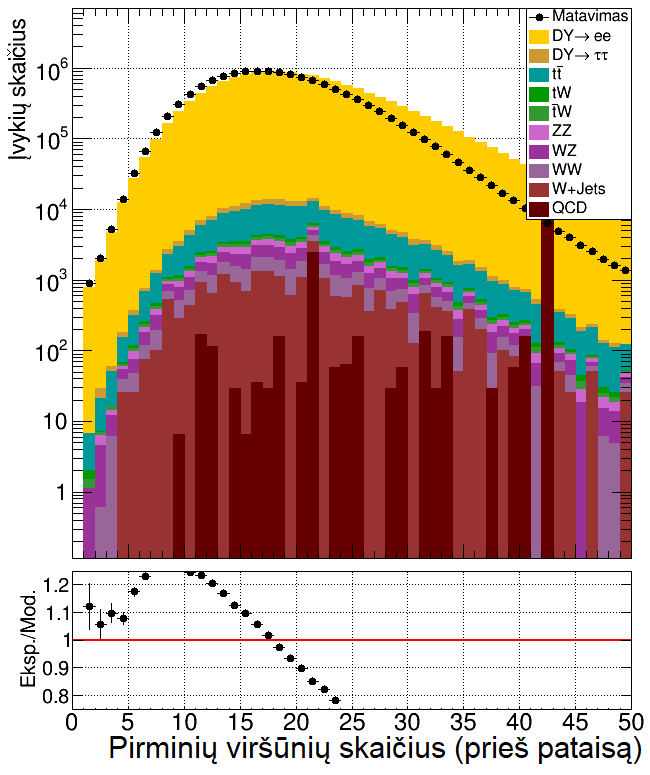
\includegraphics[width=1\linewidth]{eeNVTXbefore_SMALL.png}
	\end{minipage}
	\hfill
	\begin{minipage}[t]{0.49\linewidth}
		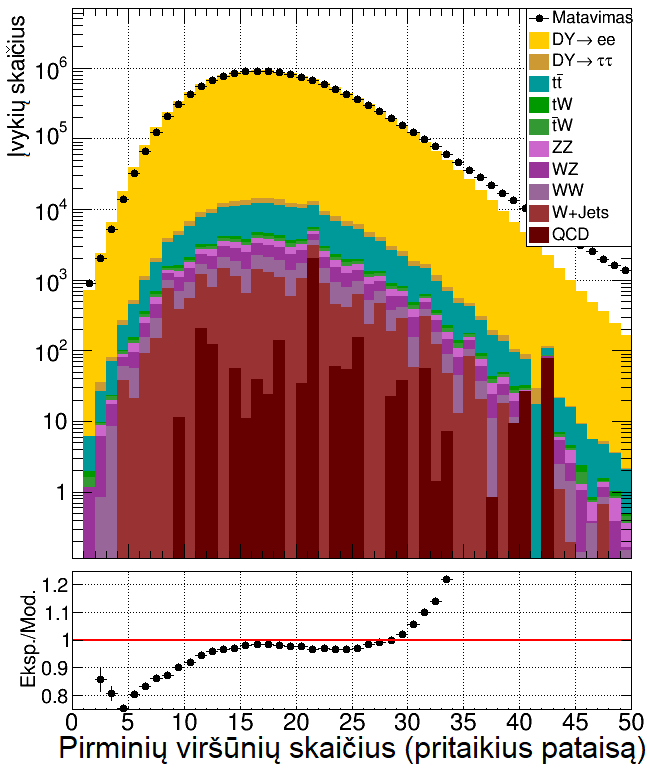
\includegraphics[width=1\linewidth]{eeNVTXafter_SMALL.png}
	\end{minipage}
	\vspace{-0.3cm}
	\captionof{figure}{\label{fig:nVTXee} \small
		Atranką praėjusiuose $ee$ įvykiuose atkurtų pirminių viršūnių skaičiaus pasiskirstymai prieš ir po pataisos, įskaitančios
		protonų susidūrimų tankio pasiskirstymų nesutapimus tarp eksperimento ir modeliavimo, pritaikymo.
		Viršutiniuose grafikuose spalvoti histogramų stulpeliai vaizduoja su skirtingais procesais siejamus modeliuotus įvykius,
		o juodi taškai -- eksperimento metu užregistruotus įvykius.
		Įvykių skaičius ant vertikalios ašies vaizduojamas logaritminėje skalėje.
		Apatiniuose grafikuose pateikiamas eksperimento ir modeliavimo santykis kiekviename histogramos stulpelyje.
		Vaizduojami neapibrėžtumai -- tik statistiniai.
	}
\end{centering}

\begin{centering}
	\begin{minipage}[t]{0.49\linewidth}
		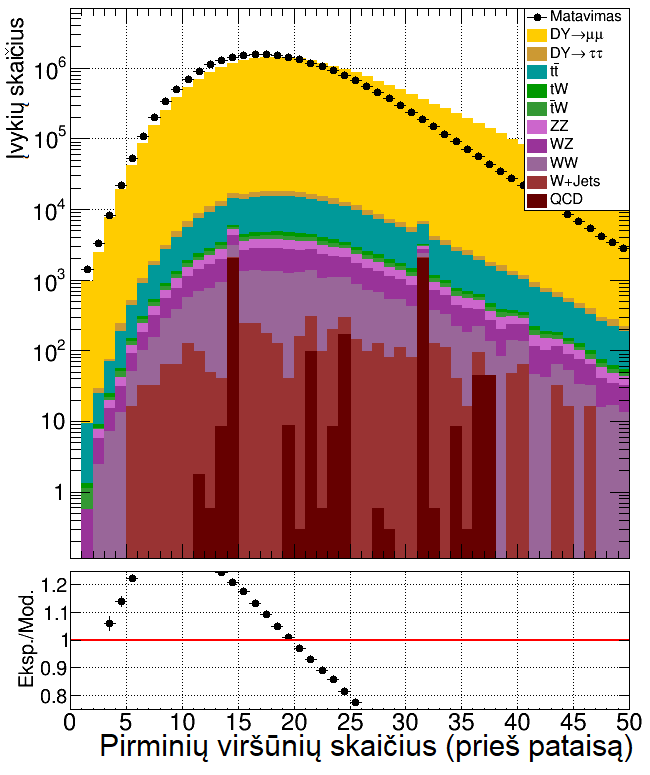
\includegraphics[width=1\linewidth]{mumuNVTXbefore_SMALL.png}
	\end{minipage}
	\hfill
	\begin{minipage}[t]{0.49\linewidth}
		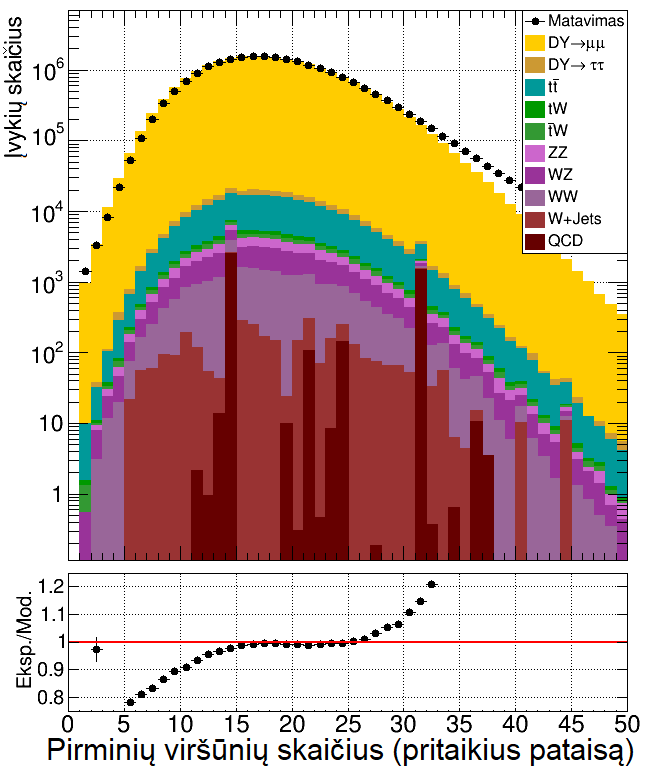
\includegraphics[width=1\linewidth]{mumuNVTXafter_SMALL.png}
	\end{minipage}
	\vspace{-0.3cm}
	\captionof{figure}{\label{fig:nVTXmumu} \small
		Atranką praėjusiuose $\mumu$ įvykiuose atkurtų pirminių viršūnių skaičiaus pasiskirstymai prieš ir po pataisos, įskaitančios
		protonų susidūrimų tankio pasiskirstymų nesutapimus tarp eksperimento ir modeliavimo, pritaikymo.
		Viršutiniuose grafikuose spalvoti histogramų stulpeliai vaizduoja su skirtingais procesais siejamus modeliuotus įvykius,
		o juodi taškai -- eksperimento metu užregistruotus įvykius.
		Įvykių skaičius ant vertikalios ašies vaizduojamas logaritminėje skalėje.
		Apatiniuose grafikuose pateikiamas eksperimento ir modeliavimo santykis kiekviename histogramos stulpelyje.
		Vaizduojami neapibrėžtumai -- tik statistiniai.
	}
	\vspace{0.6cm}
\end{centering}

Kitos taikytos pataisos buvo aprašytos \ref{sec:SFs} skyrelyje.
Elektronų ir miuonų porų invariantinės masės histogramos pateikiamos atitinkamai \ref{fig:eeMassSF} ir \ref{fig:mumuMassSF}
paveiksluose.
Juose pateikiamas išmatuoto ir sumodeliuoto rezultato palyginimas prieš ir po minėtų pataisų taikymo.
\ref{fig:eeMassSF} paveiksle prieš korekcijų pritaikymą nesutapimas tarp matavimo ir modeliavimo buvo apie $15.1\%$, o
\ref{fig:mumuMassSF} -- apie $6.3\%$.
Po visų pataisų pritaikymo rezultatas akivaizdžiai pagerėjo -- skirtumas tarp eksperimento ir modeliavimo $ee$ įvykiams
tapo lygus apie $2.5\%$, $\mumu$ įvykiams -- apie $1.0\%$.
Taigi, pataisų taikymas buvo naudingas.

\begin{centering}
	\vspace{0.6cm}
	\begin{minipage}[t]{0.49\linewidth}
		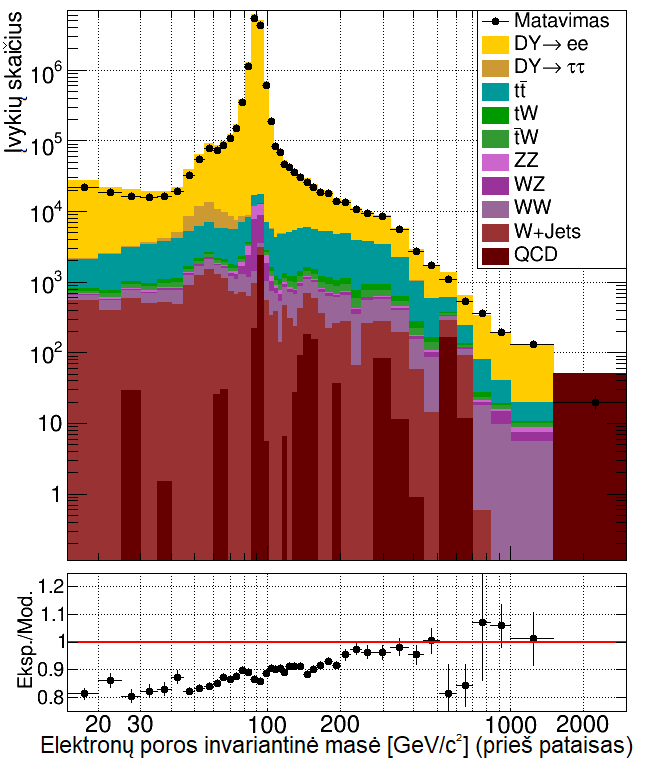
\includegraphics[width=1\linewidth]{eeMassBefore_SMALL.png}
	\end{minipage}
	\hfill
	\begin{minipage}[t]{0.49\linewidth}
		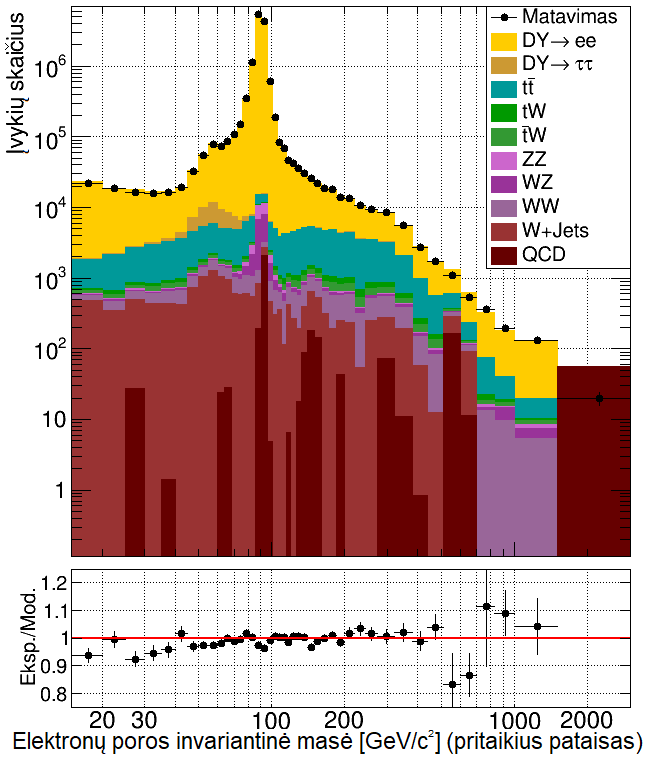
\includegraphics[width=1\linewidth]{eeMassAfter_SMALL.png}
	\end{minipage}
	\vspace{-0.3cm}
	\captionof{figure}{\label{fig:eeMassSF} \small
		Elektronų poros invariantinės masės pasiskirstymo histogramos prieš ir po efektyvumų pataisų pritaikymo.
		Viršutiniuose grafikuose spalvoti histogramų stulpeliai vaizduoja su skirtingais procesais siejamus modeliuotus įvykius,
		o juodi taškai -- eksperimento metu užregistruotus įvykius.
		Skalės -- logaritminės.
		Apatiniuose grafikuose pateikiamas eksperimento ir modeliavimo santykis kiekviename histogramos stulpelyje.
		Vaizduojami neapibrėžtumai -- tik statistiniai.
	}
\end{centering}

\begin{centering}
	\begin{minipage}[t]{0.49\linewidth}
		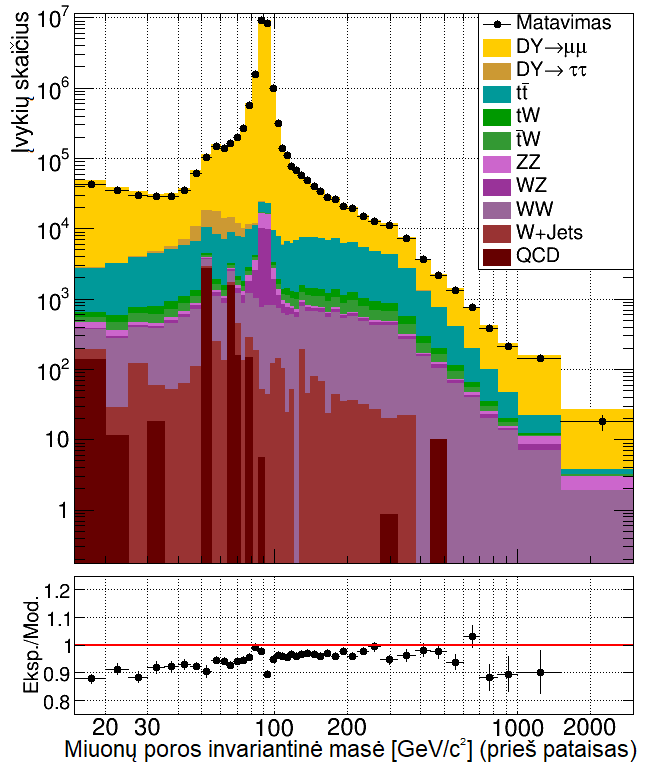
\includegraphics[width=1\linewidth]{mumuMassBefore_SMALL.png}
	\end{minipage}
	\hfill
	\begin{minipage}[t]{0.49\linewidth}
		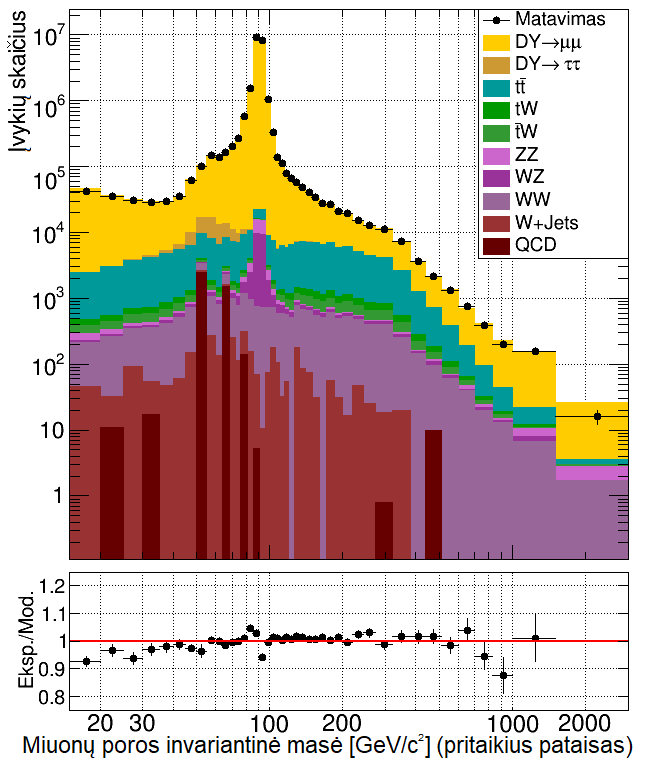
\includegraphics[width=1\linewidth]{mumuMassAfter_SMALL.png}
	\end{minipage}
	\vspace{-0.3cm}
	\captionof{figure}{\label{fig:mumuMassSF} \small
		Miuonų poros invariantinės masės pasiskirstymo histogramos prieš ir po efektyvumų pataisų pritaikymo.
		Viršutiniuose grafikuose spalvoti histogramų stulpeliai vaizduoja su skirtingais procesais siejamus modeliuotus įvykius,
		o juodi taškai -- eksperimento metu užregistruotus įvykius.
		Skalės -- logaritminės.
		Apatiniuose grafikuose pateikiamas eksperimento ir modeliavimo santykis kiekviename histogramos stulpelyje.
		Vaizduojami neapibrėžtumai -- tik statistiniai.
	}
\end{centering}


\subsection{Netikrų $e\mu$ įvykių skaičiaus įvertinimas}

Drell-Yan proceso triukšmo įvykių skaičiaus įvertinimui $\emu$ metodu buvo atrinkti eksperimento metu užregistruoti bei
modeliuoti elektrono ir miuono galutinės būsenos įvykiai.
$\emu$ triukšmo -- $\QCD$ -- įvykių skaičius buvo įvertinti pasinaudojant tokiais įvykiais, kuriuose buvo užregistruoti
vienodą elektrinį krūvį turintys elektronas ir miuonas.
Priešingus elektrinius krūvius turinčių elektrono ir miuono invariantinės masės histograma vaizduojama \ref{fig:emuOS}
pav., o vienodus krūvius turinčių elektrono ir miuono -- \ref{fig:emuSS} paveiksle.
Histogramos pavaizduotos pritaikius tokias pačias pataisas, kaip ir aprašytosios praeitame skyrelyje.

\ref{fig:emuOS} pav.\ histogramoje nesutapimas tarp eksperimento metu užregistruotų ir sumodeliuotų įvykių skaičiaus siekia
apie $0.7\%$ (čia kalbama apie pilnutinį įvykių skaičių; lyginant matavimą ir modeliavimą kiekviename histogramos stulpelyje
atskirai skirtumai, priklausomai nuo stulpelio, gali būti ir gerokai didesni), o \ref{fig:emuSS} paveiksle, kuriame
vaizduojamas įvykių su vienodo krūvio dalelėmis skaičius, šis nesutapimas yra žymiai didesnis -- apie $64.4\%$.
To ir buvo tikimasi, nes į minimą histogramą nebuvo įtraukti modeliuoti $\emu$ triukšmo įvykiai.
Jų skaičiumi ir yra laikomas visas grafike matomas skirtumas tarp matavimo ir modeliavimo.
Šio skirtumo vertė buvo transformuojama į $\emu$ triukšmo įvykių skaičių priešingo krūvio dalelių (signalo) srityje pagal
\ref{sec:emu} skyrelyje aprašytą metodiką.

\begin{figure}[H]
	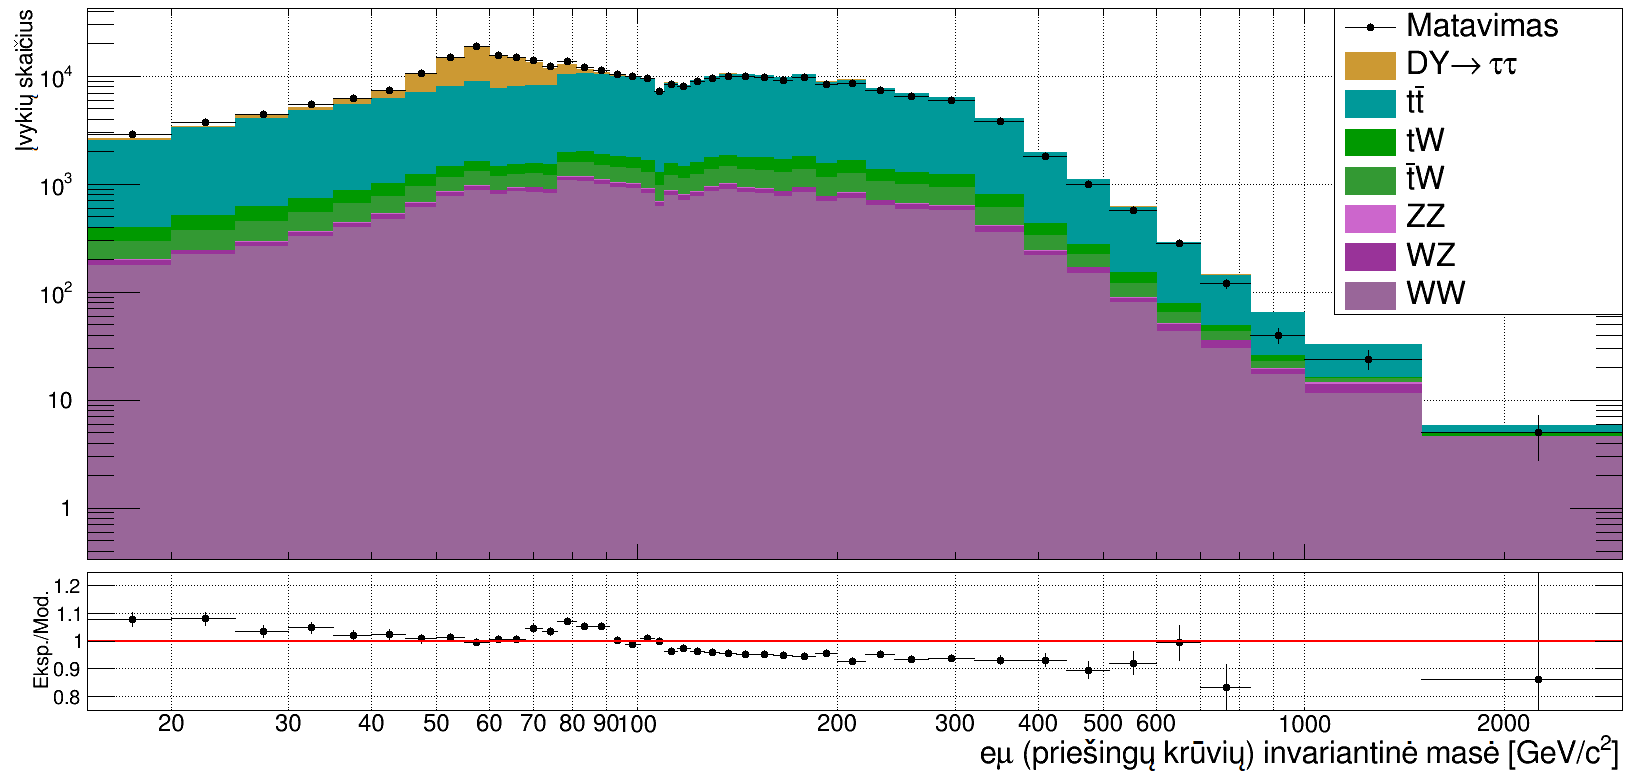
\includegraphics[width=\linewidth]{emuMassOS_BIG.png}
	\caption{\label{fig:emuOS} \small
		Priešingus elektrinius krūvius turinčių elektrono ir miuono invariantinės masės pasiskirstymo histograma.
		Viršutiniuose grafikuose spalvoti histogramų stulpeliai vaizduoja su skirtingais procesais siejamus modeliuotus įvykius,
		o juodi taškai -- eksperimento metu užregistruotus įvykius.
		Skalės -- logaritminės.
		Apatiniuose grafikuose pateikiamas eksperimento ir modeliavimo santykis kiekviename histogramos stulpelyje.
		Vaizduojami neapibrėžtumai -- tik statistiniai.
	}
\end{figure}

\begin{figure}[H]
	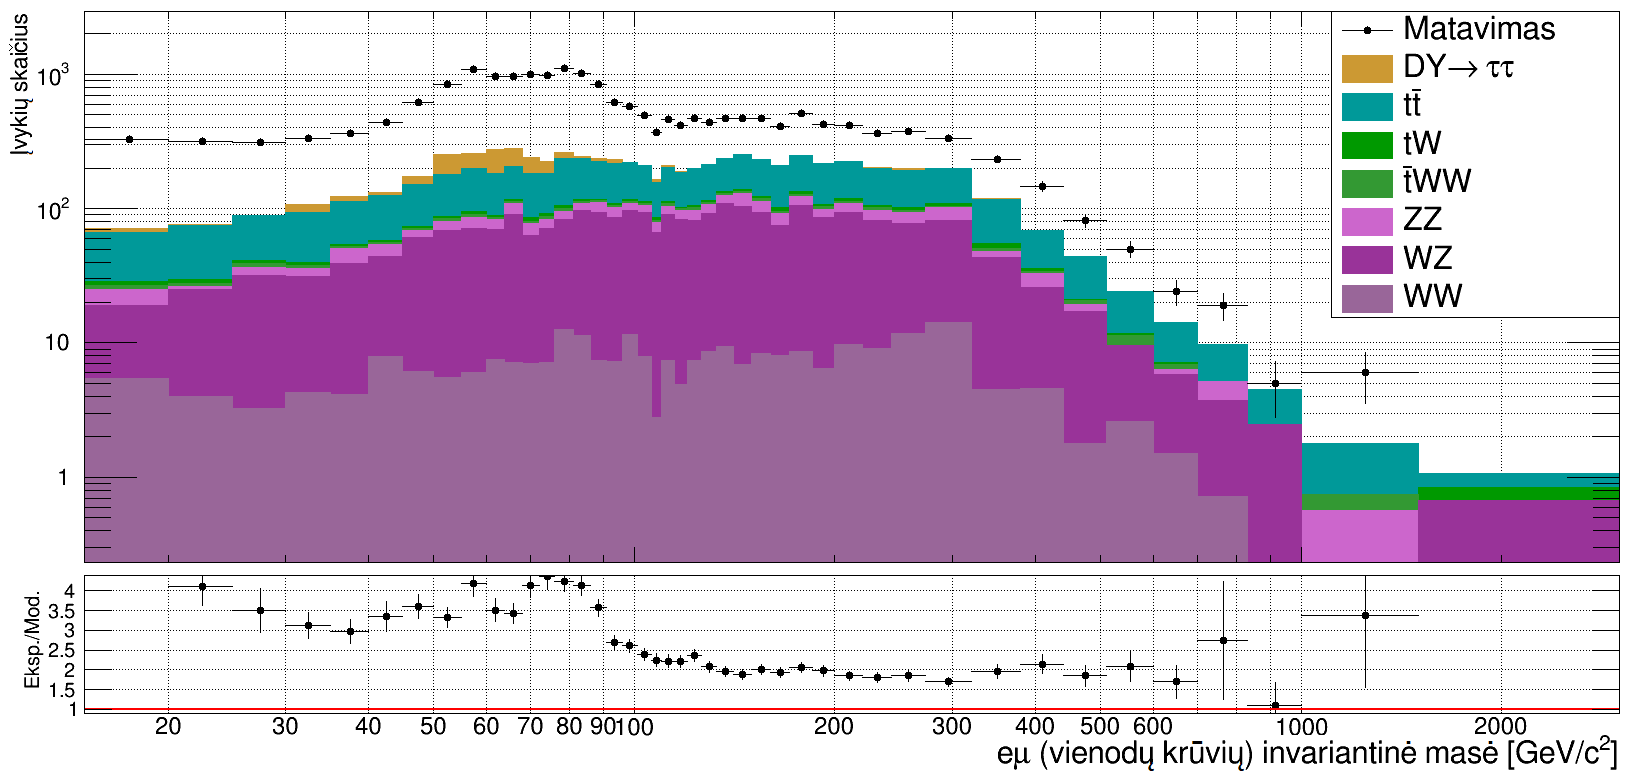
\includegraphics[width=\linewidth]{emuMassSS_BIG.png}
	\caption{\label{fig:emuSS} \small
		Sutampančius elektrinius krūvius turinčių elektrono ir miuono invariantinės masės pasiskirstymo histograma.
		Viršutiniuose grafikuose spalvoti histogramų stulpeliai vaizduoja su skirtingais procesais siejamus modeliuotus įvykius,
		o juodi taškai -- eksperimento metu užregistruotus įvykius.
		Skalės -- logaritminės.
		Šioje histogramoje visas skirtumas tarp eksperimentinio ir modeliuoto rezultato bus traktuojamas kaip susijęs su
		$\QCD$ procesu.
		Apatiniuose grafikuose pateikiamas eksperimento ir modeliavimo santykis kiekviename histogramos stulpelyje.
		Vaizduojami neapibrėžtumai -- tik statistiniai.
	}
\end{figure}

\begin{figure}[H]
	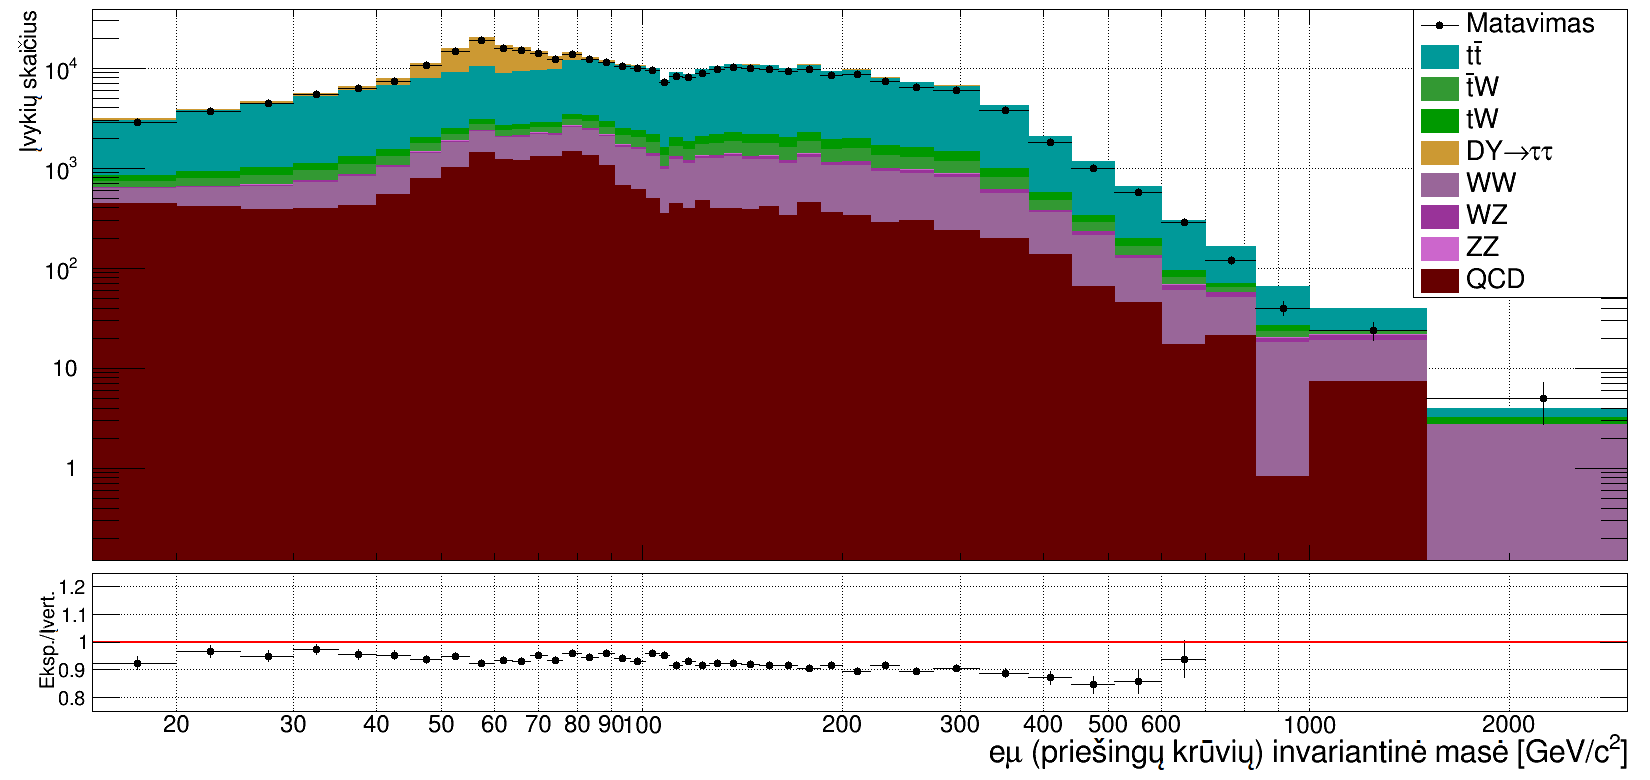
\includegraphics[width=\linewidth]{emuWQCD_BIG.png}
	\caption{\label{fig:emuWQCD} \small
		Priešingus elektrinius krūvius turinčių elektrono ir miuono invariantinės masės pasiskirstymo histograma, įskaičius
		$\QCD$ triukšmo egzistavimą.
		Viršutiniuose grafikuose spalvoti histogramų stulpeliai vaizduoja su skirtingais procesais siejamus modeliuotus įvykius,
		bei $\QCD$ įvykius, įvertintus iš matavimo, o juodi taškai -- eksperimento metu užregistruotus įvykius.
		Skalės -- logaritminės.
		Apatiniuose grafikuose pateikiamas eksperimento ir modeliavimo bei $\QCD$ įverčio santykis kiekviename histogramos stulpelyje.
		Vaizduojami neapibrėžtumai -- tik statistiniai.
	}
\end{figure}

Priešingus elektrinius krūvius turinčių elektrono ir miuono invariantinės masės histograma, pridėjus iš vienodo krūvio srities
įvertintus $\QCD$ įvykius, vaizduojama \ref{fig:emuWQCD} paveiksle.
Šiuo atveju skirtumas tarp matavimo ir modeliavimo, pridėjus $\QCD$ įvykius, siekia apie $8.0\%$.
Iš įnešto sistemingo nuokrypio galima spręsti, kad tokia netikrų $\emu$ įvykių skaičiaus įvertinimo metodika turi trūkumų ir ją
reikėtų patobulinti, arba pabandyti taikyti kitą metodiką.

\subsection{Išmatuotas invariantinės masės pasiskirstymas}

$\emu$ metodu buvo vertinamas Drell-Yan proceso triukšmo įvykių skaičius tiek $ee$, tiek $\mumu$ galutinėse būsenose.
Skaičiavimai buvo atliekami kiekvienam histogramos stulpeliui atskirai, naudojantis \eqref{eq:emuFinal} formule.
Triukšmo įvykių skaičiaus įverčiai, gauti $\emu$ metodu, invariantinės masės histogramų pavidaluose pateikiami
\ref{fig:eeEst} paveiksle $ee$ kanalui ir \ref{fig:mumuEst} paveiksle $\mumu$ kanalui.
Šiuose paveiksluose taip pat pateikiami įverčių ir modeliavimo palyginimai.
Galima pastebėti, kad įverčio ir modeliuoto rezultato santykio, pateikiamo paveikslų apačiose forma yra vienoda, bei
sutampa su matavimo ir modeliavimo (pridėjus $\QCD$ įvykių skaičiaus įvertį) forma, matoma \ref{fig:emuWQCD} paveiksle.
Taip yra dėl jau aprašytos \eqref{eq:emuFinal} formulės specifikos.
Taikant $\emu$ metodą gautų įvykių skaičių neapibrėžtumai buvo įvertinti naudojantis \ref{eq:DerUnc} formule.

\begin{figure}[H]
	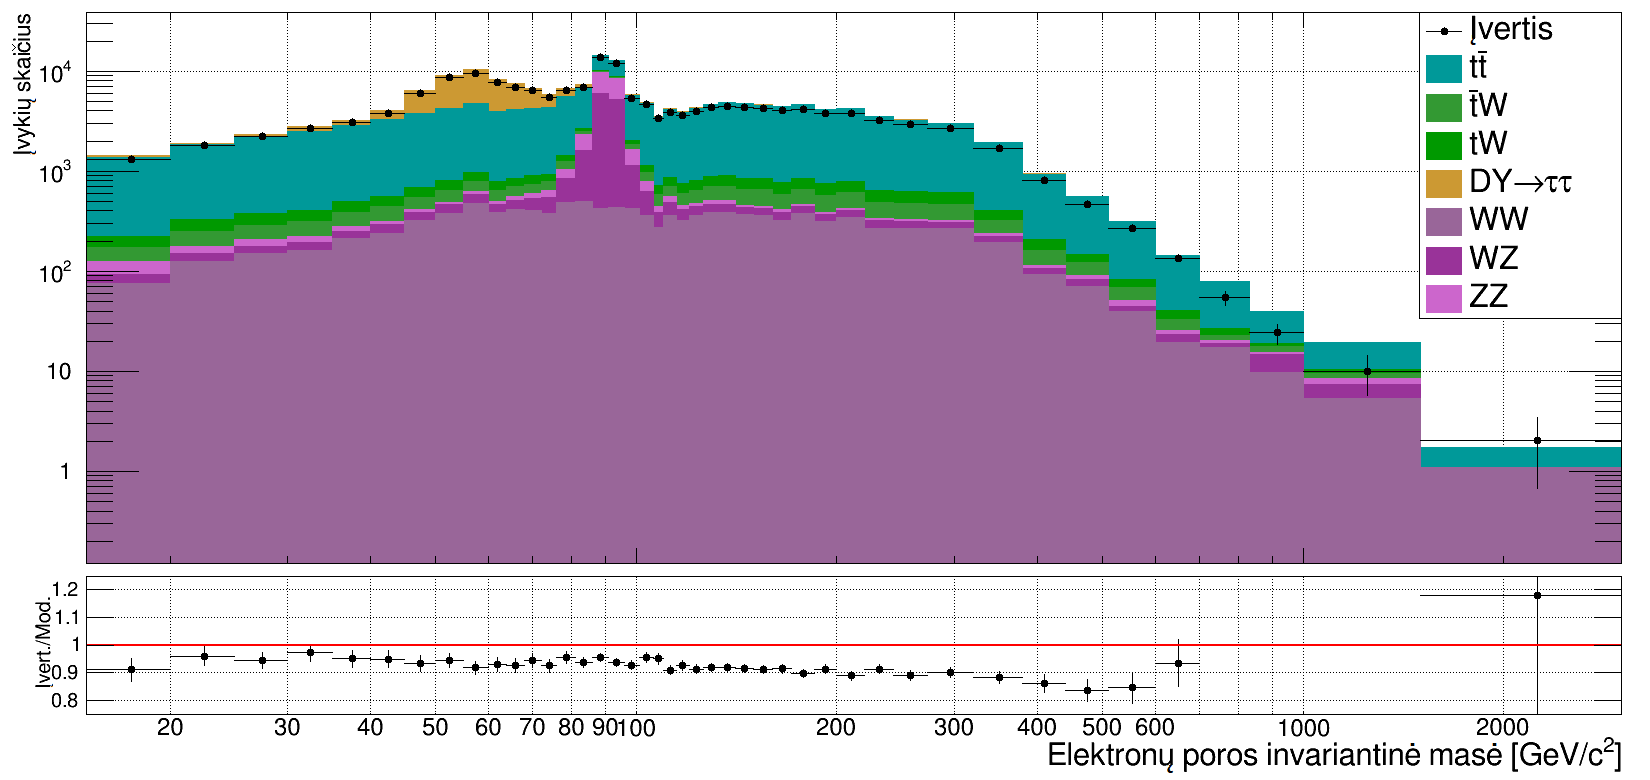
\includegraphics[width=\linewidth]{eeMassEst_BIG.png}
	\caption{\label{fig:eeEst} \small
		Su Drell-Yan triukšmo procesais siejamos elektronų poros invariantinės masės pasiskirstymo histograma.
		Viršutiniuose grafikuose spalvoti histogramų stulpeliai vaizduoja su skirtingais procesais siejamus modeliuotus įvykių
		skaičius, o juodi taškai -- $\emu$ metodu apskaičiuotus įvykių skaičius.
		Skalės -- logaritminės.
		Apatiniuose grafikuose pateikiamas $\emu$ metodo įverčio ir modeliavimo santykis kiekviename histogramos stulpelyje.
		Vaizduojami neapibrėžtumai -- tik statistiniai.
	}
\end{figure}

\begin{figure}[H]
	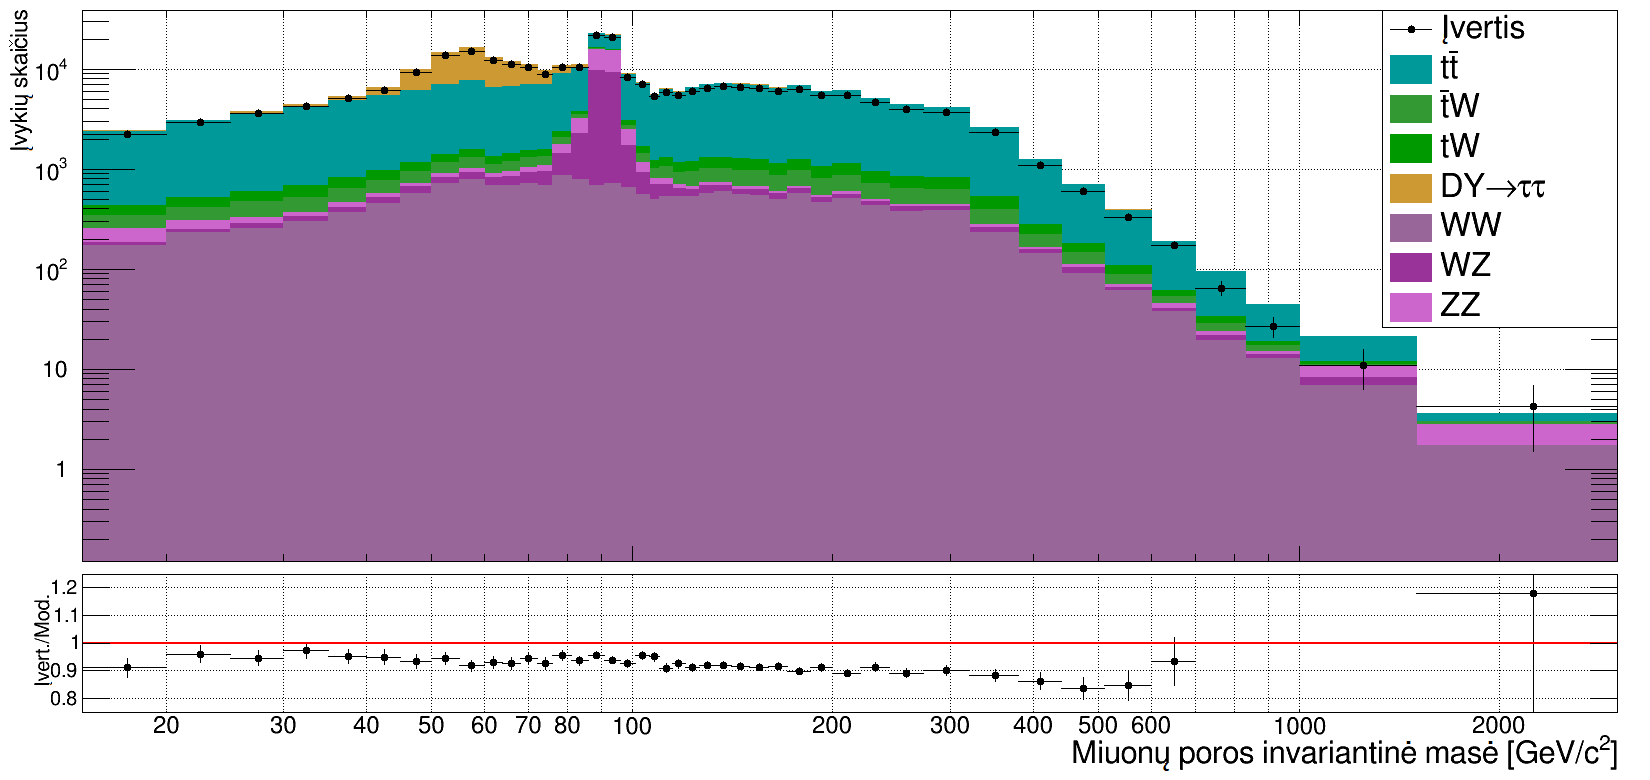
\includegraphics[width=0.9\linewidth]{mumuMassEst_BIG.png}
	\vspace{-0.4cm}
	\caption{\label{fig:mumuEst} \small
		Su Drell-Yan triukšmo procesais siejamos miuonų poros invariantinės masės pasiskirstymo histograma.
		Viršutiniuose grafikuose spalvoti histogramų stulpeliai vaizduoja su skirtingais procesais siejamus modeliuotus įvykių
		skaičius, o juodi taškai -- $\emu$ metodu apskaičiuotus įvykių skaičius.
		Skalės -- logaritminės.
		Apatiniuose grafikuose pateikiamas $\emu$ metodo įverčio ir modeliavimo santykis kiekviename histogramos stulpelyje.
		Vaizduojami neapibrėžtumai -- tik statistiniai.
	}
\end{figure}
\vspace{-0.4cm}

\ref{fig:eeMassDataMCest} bei \ref{fig:mumuMassDataMCest} paveiksluose pateikiamos leptonų porų invariantinių masių
histogramos, kuriose $\DYtau$, $\ttbar$, $tW$, $\tbarW$, $WW$, $WZ$ ir $ZZ$ procesų modeliuoti įverčiai yra pakeisti
į gautuosius naudojant $\emu$ metodą.
Taip pat $\emu$ metodo pritaikymo rezultatai kartu su statistiniais neapibrėžtumais pateikiami
\ref{table:finalResults_Full} ir \ref{table:finalResults_Z} lentelėse. \ref{table:finalResults_Full} lentelėje pateikiami įvykių
skaičiai visoje tirtoje invariantinės masės srityje, \ref{table:finalResults_Z} lentelėje -- $Z$ bozono rezonanso aplinkoje
($15<m_{ll}<3000$ GeV).
Lyginant su vien tik iš modeliavimo įvertintą įvykių skaičių su gautuoju taikant $\emu$ metodą (lentelių 3-asis ir 4-asis stulpeliai),
skirtumas tarp pilnutinio (suintegruoto visoje tirtoje invariantinės masės srityje) išmatuoto ir modeliavimu arba $\emu$ metodu gauto
įverčio šiek tiek sumažėjo: $ee$ galutinės būsenos įvykiams nuo $2.54\%$ iki $2.43\%$, o $\mumu$ įvykiams -- nuo $1.01\%$ iki $0.92\%$.
Šis pasikeitimas atrodo nežymus, nes $\emu$ metodu įvertinamas ne visų triukšmo įvykių skaičius, o svarbiausia --
signalo srityje labai didelę dalį įvykių ir sudaro pats signalas: apie $98.5\%$ visų įvykių.
Vis dėlto, kadangi $\emu$ metodu įvertintas Drell-Yan triukšmo įvykių skaičius yra net $8\%$ mažesnis už modeliuotų triukšmo įvykių
skaičių, galima manyti, kad $\emu$ metodas įvykių skaičių sumažino per smarkiai.
Tokį įvykių skaičiaus pasikeitimą nulėmė išbandyta netikrų $\emu$ įvykių skaičiaus įvertinimo metodika, kuri šiuo atveju pasirodė netinkama.

\begin{figure}
	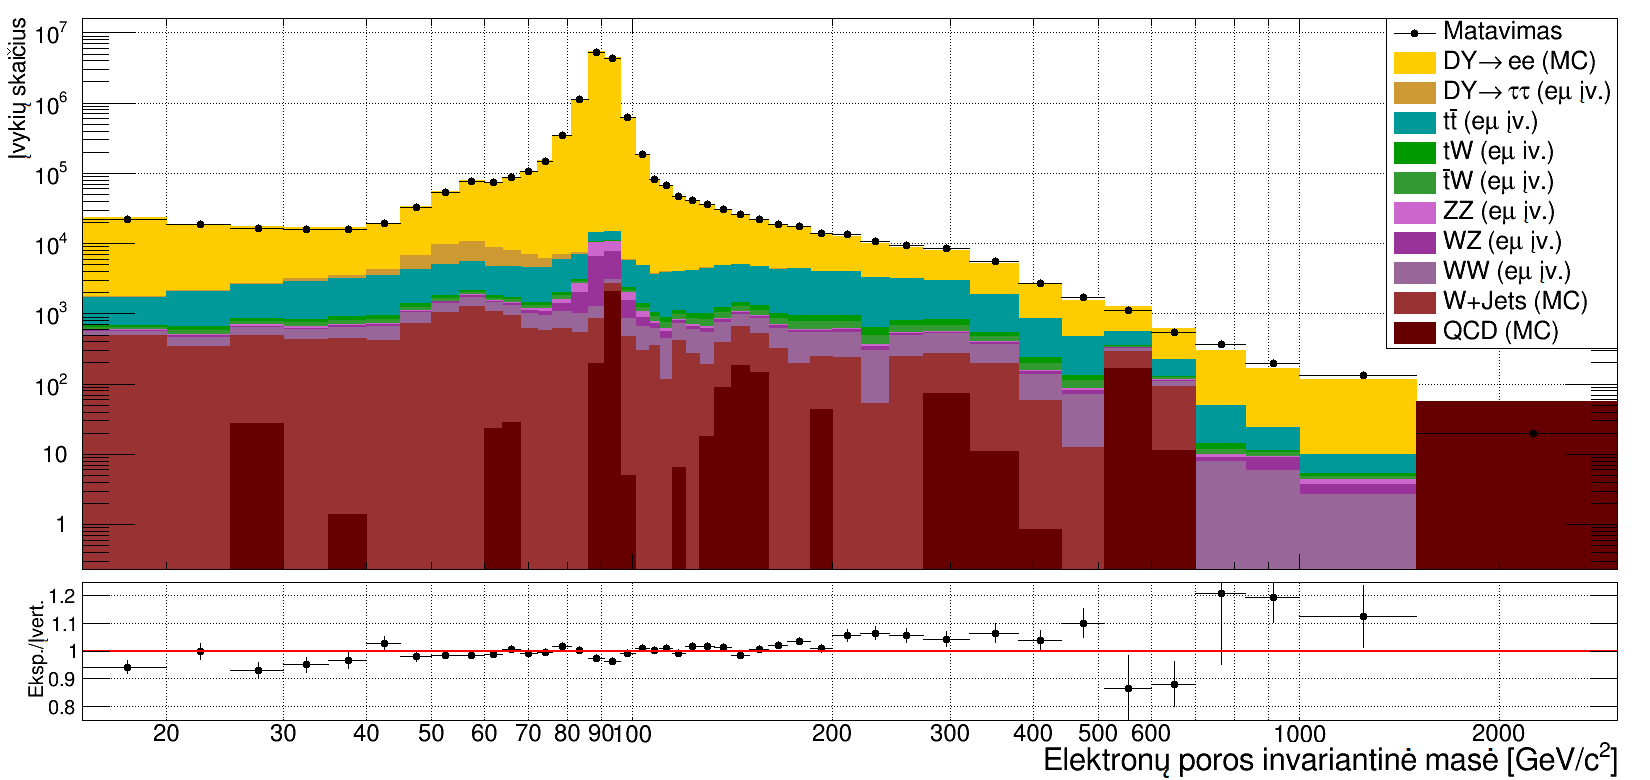
\includegraphics[width=\linewidth]{eeMassFinal_BIG.png}
	\vspace{-0.8cm}
	\caption{\label{fig:eeMassDataMCest} \small
		Elektronų poros invariantinės masės pasiskirstymo histograma, kurioje, kur įmanoma, modeliuotų įvykių skaičius yra
		pakeistas $\emu$ metodu įvertintu įvykių skaičiumi. 
		Viršutiniuose grafikuose spalvoti histogramų stulpeliai vaizduoja su skirtingais procesais siejamus modeliuotus įvykių
		skaičius (legendoje žymima \ltq{MC}, bei $\emu$ metodu įvertintus įvykių skaičius (legendoje žymima \ltq{$\emu$ įv.}),
		o juodi taškai -- eksperimento metu užregistruotus įvykius.
		Skalės -- logaritminės.
		Apatiniuose grafikuose pateikiamas eksperimento ir modeliavimo bei $\emu$ metodo įverčio santykis kiekviename
		histogramos stulpelyje.
		Vaizduojami neapibrėžtumai -- tik statistiniai.
	}
\end{figure}

\begin{figure}
	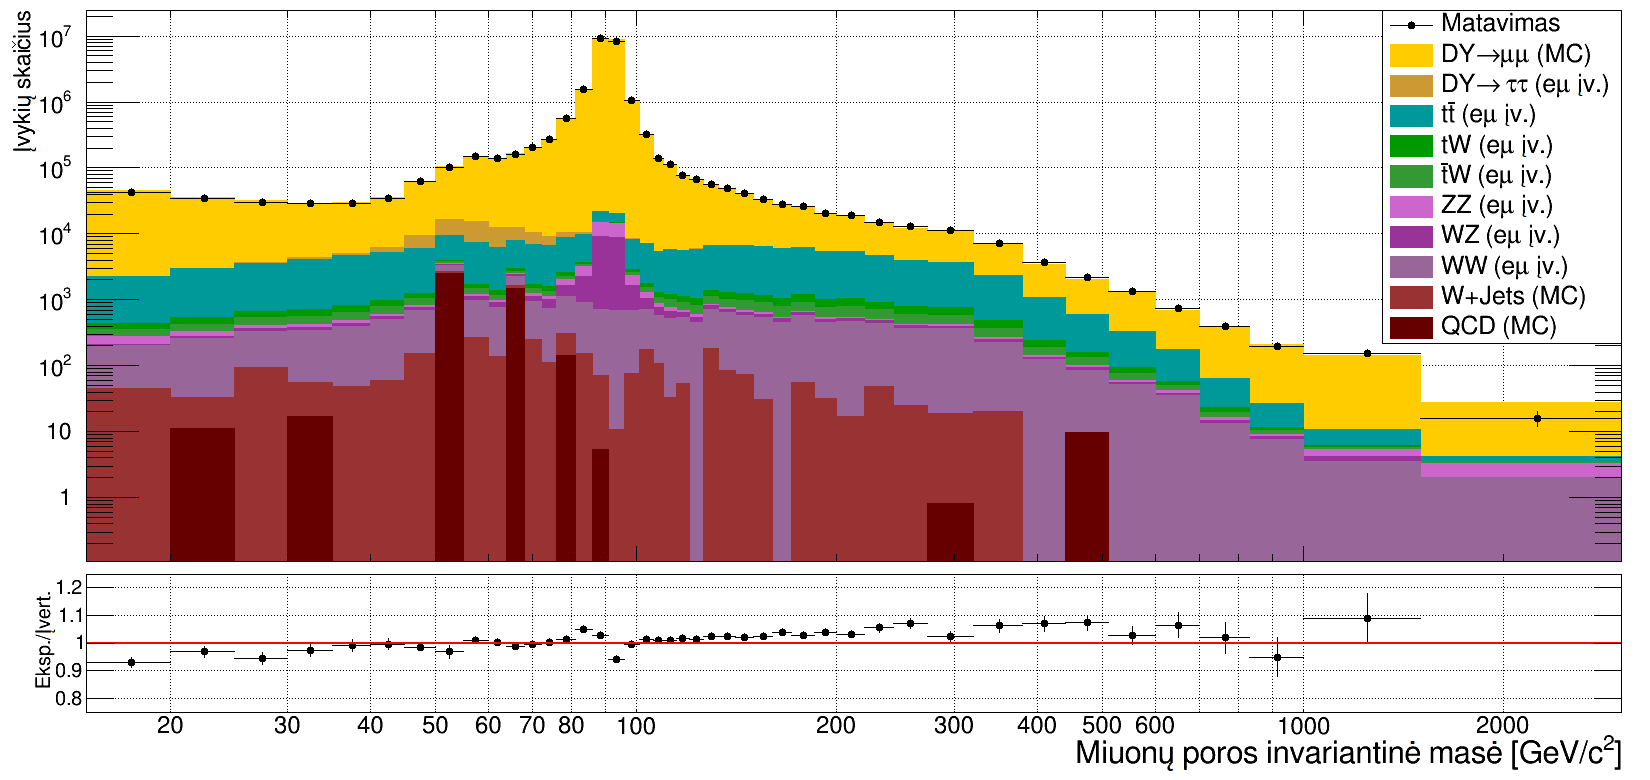
\includegraphics[width=\linewidth]{mumuMassFinal_BIG.png}
	\vspace{-0.8cm}
	\caption{\label{fig:mumuMassDataMCest} \small
		Miuonų poros invariantinės masės pasiskirstymo histograma, kurioje, kur įmanoma, modeliuotų įvykių skaičius yra
		pakeistas $\emu$ metodu įvertintu įvykių skaičiumi. 
		Viršutiniuose grafikuose spalvoti histogramų stulpeliai vaizduoja su skirtingais procesais siejamus modeliuotus įvykių
		skaičius (legendoje žymima \ltq{MC}, bei $\emu$ metodu įvertintus įvykių skaičius (legendoje žymima \ltq{$\emu$ įv.}),
		o juodi taškai -- eksperimento metu užregistruotus įvykius.
		Skalės -- logaritminės.
		Apatiniuose grafikuose pateikiamas eksperimento ir modeliavimo bei $\emu$ metodo įverčio santykis kiekviename
		histogramos stulpelyje.
		Vaizduojami neapibrėžtumai -- tik statistiniai.
	}
\end{figure}

Drell-Yan proceso triukšmo įvykių skaičiaus neapibrėžtumas, lyginant su modeliavimu, išaugo daugiau negu $50\%$.
Taip yra dėl to, kad įvykių skaičius, apskaičiuojamas $\emu$ metodu yra išvestinis dydis, gaunamas iš \eqref{eq:emuFinal}
formulės, o jo neapibrėžtumas įvertinamas naudojantis \eqref{eq:DerUnc} formule.

Nors $\emu$ metodas leido įvertinti Drell-Yan proceso triukšmo įvykių skaičių, ateityje metodiką reikės patobulinti.
Tikslingiausia būtų pabandyti $\emu$ triukšmo įvykių skaičių įvertinti kitais matavimu grįstais metodais.

\begin{centering}
\begin{table}[H]
	\small
\begin{tabular}{|c|c|c|c|} %|p{5cm}|p{4cm}|p{8cm}|p{9cm}|
	\hline
	
	\multirow{2}{8em}{\centering Įvykiai} &
	\multirow{2}{8em}{\centering CMS užfiksuotų įvykių skaičius} &
	\multirow{2}{9em}{\centering Modeliuotų įvykių skaičius} &
	\multirow{2}{10em}{\centering Įvykių skaičius, gautas taikant $e\mu$ metodą} \\
	
 	& & & \\
	\hline \hline
	
	\multirow{2}{8em}{\centering $e\mu$} &
	\multirow{2}{8em}{\centering $(3.110 \pm 0.006) \cdot 10^5$} &
	\multirow{2}{9em}{\centering $(3.359 \pm 0.005) \cdot 10^5$ } &
	\multirow{2}{5em}{\centering \textendash }\\
	
 	& & & \\
	\hline
	
	$ee$ ($\WW$, $tW$, $\bar{t}W$, &
	\multirow{2}{8em}{\centering\textendash} &
	\multirow{2}{9em}{\centering $(1.883 \pm 0.004) \cdot 10^5$} &
	\multirow{2}{9em}{\centering$\mathbf{(1.749 \pm 0.006) \cdot 10^5}$} \\
	
	$t\bar{t}$, $\DYtau$) & & & \\
	\hline
	
	\multirow{2}{8em}{\centering $ee$ (visi procesai)} &
	\multirow{2}{8em}{\centering $(1.311 \pm 0) \cdot 10^7$} &
	\multirow{2}{10em}{\centering $(1.344 \pm 0.001) \cdot 10^7$}
	&\multirow{2}{10em}{\centering $\mathbf{(1.343 \pm 0.001) \cdot 10^7}$} \\
	
 	& & & \\
	\hline

	\multirow{2}{8em}{\centering $N_{ee}/N_{ee}^{\mathrm{Obs.}}$} &
	\multirow{2}{8em}{\centering \textendash} &
	\multirow{2}{10em}{\centering $1.0254 \pm 0.0006$} &
	\multirow{2}{10em}{\centering $1.0243 \pm 0.0006$} \\
	
 	& & & \\
	\hline

	$\mumu$ ($\WW$, $tW$, $\bar{t}W$, &
	\multirow{2}{8em}{\centering\textendash} &
	\multirow{2}{9em}{\centering $(2.931 \pm 0.005) \cdot 10^5$} &
	\multirow{2}{9em}{\centering$\mathbf{(2.724 \pm 0.009) \cdot 10^5}$} \\
	
	$t\bar{t}$, $\DYtau$) & & & \\
	\hline
	
	\multirow{2}{8em}{\centering $\mumu$ (visi procesai)} &
	\multirow{2}{8em}{\centering $(2.292 \pm 0) \cdot 10^7$} &
	\multirow{2}{10em}{\centering $(2.315 \pm 0.001) \cdot 10^7$}
	&\multirow{2}{10em}{\centering $\mathbf{(2.313 \pm 0.001) \cdot 10^7}$} \\
	
 	& & & \\
	\hline
	
	\multirow{2}{8em}{\centering $N_{\mumu}/N_{\mumu}^{\mathrm{Obs.}}$} &
	\multirow{2}{8em}{\centering \textendash} &
	\multirow{2}{10em}{\centering $1.0101 \pm 0.0005$} &
	\multirow{2}{10em}{\centering $1.0092 \pm 0.0005$} \\
	
 	& & & \\
	\hline
\end{tabular}
	\caption{\label{table:finalResults_Full} \small
	CMS detektoriaus užregistruotų, modeliuotų, bei $\emu$ metodu įvertintų įvykių skaičiai bei jų statistinės
	paklaidos visoje tirtoje leptonų poros invariantinės masės srityje ($15<m_{ll}<3000$ GeV).}
\end{table}
\end{centering}

\begin{centering}
\begin{table}[H]
	\small
\begin{tabular}{|c|c|c|c|} %|p{5cm}|p{4cm}|p{8cm}|p{9cm}|
	\hline
	
	\multirow{2}{8em}{\centering Įvykiai} &
	\multirow{2}{8em}{\centering CMS užfiksuotų įvykių skaičius} &
	\multirow{2}{9em}{\centering Modeliuotų įvykių skaičius} &
	\multirow{2}{10em}{\centering Įvykių skaičius, gautas taikant $e\mu$ metodą} \\
	
 	& & & \\
	\hline \hline
	
	\multirow{2}{8em}{\centering $e\mu$} &
	\multirow{2}{8em}{\centering $(1.357 \pm 0.004) \cdot 10^5$} &
	\multirow{2}{9em}{\centering $(1.449 \pm 0.004) \cdot 10^5$ } &
	\multirow{2}{5em}{\centering \textendash }\\
	
 	& & & \\
	\hline
	
	$ee$ ($\WW$, $tW$, $\bar{t}W$, &
	\multirow{2}{8em}{\centering\textendash} &
	\multirow{2}{9em}{\centering $92178 \pm 288$} &
	\multirow{2}{9em}{\centering $\mathbf{86510} \pm 455$} \\
	
	$t\bar{t}$, $\DYtau$) & & & \\
	\hline
	
	\multirow{2}{8em}{\centering $ee$ (visi procesai)} &
	\multirow{2}{8em}{\centering $(1.257 \pm 0) \cdot 10^7 $} &
	\multirow{2}{10em}{\centering $(1.290 \pm 0.001) \cdot 10^7$} &
	\multirow{2}{10em}{\centering $\mathbf{(1.289 \pm 0.001) \cdot 10^7}$} \\
	
 	& & & \\
	\hline

	\multirow{2}{8em}{\centering $N_{ee}/N_{ee}^{\mathrm{Obs.}}$} &
	\multirow{2}{8em}{\centering\textendash} &
	\multirow{2}{10em}{\centering $1.0262 \pm 0.0006$} &
	\multirow{2}{10em}{\centering $1.0255 \pm 0.0006$} \\
	
 	& & & \\
	\hline

	$\mumu$ ($\WW$, $tW$, $\bar{t}W$, &
	\multirow{2}{8em}{\centering\textendash} &
	\multirow{2}{9em}{\centering $(1.469 \pm 0.004) \cdot 10^5$} &
	\multirow{2}{9em}{\centering$\mathbf{(1.379 \pm 0.007) \cdot 10^5}$} \\
	
	$t\bar{t}$, $\DYtau$) & & & \\
	\hline
	
	\multirow{2}{8em}{\centering $\mumu$ (visi procesai)} &
	\multirow{2}{8em}{\centering $(2.201 \pm 0) \cdot 10^7$} &
	\multirow{2}{10em}{\centering $(2.223 \pm 0.001) \cdot 10^7$} &
	\multirow{2}{10em}{\centering $\mathbf{(2.222 \pm 0.001) \cdot 10^7}$} \\
	
 	& & & \\
	\hline
	
	\multirow{2}{8em}{\centering $N_{\mumu}/N_{\mumu}^{\mathrm{Obs.}}$} &
	\multirow{2}{8em}{\centering \textendash} &
	\multirow{2}{10em}{\centering $1.0100 \pm 0.0005$} &
	\multirow{2}{10em}{\centering $1.0095 \pm 0.0005$} \\
	
 	& & & \\
	\hline
\end{tabular}
	\caption{\label{table:finalResults_Z} \small
	CMS detektoriaus užregistruotų, modeliuotų, bei $\emu$ metodu įvertintų įvykių skaičiai	bei jų statistinės
	paklaidos su $Z$ bozono rezonansu siejamoje leptonų poros invariantinės masės srityje ($60<m_{ll}<120$ GeV).}
\end{table}
\end{centering}


\clearpage
\section*{Išvados} \addcontentsline{toc}{section}{Išvados}
\begin{enumerate}
	\item Duomenų rinkinių sukūrimas, saugant tik atranką praėjusius įvykius, gerokai sutrumpina tolimesnės duomenų analizės
	laiką bei supaprastina duomenų saugojimą;
	\item Į eksperimento ir modeliavimo sąlygų nesutapimus atsižvelgiančios pataisos padeda sumažinti atranką praeinančių
	išmatuotų ir modeliuotų įvykių skaičiaus neatitikimus;
	\item Iš matavimo duomenų įvertinus netikrus $\emu$ įvykius galima geriau įvertinti $\emu$ įvykių skaičių, tačiau pritaikytas
	metodas nepasiteisino ir turi būti peržiūrėtas;
	\item $\emu$ metodas leidžia įvertinti Drell-Yan proceso triukšmo įvykių skaičių, bet galutinę metodiką dar reikia patobulinti.
\end{enumerate}

\clearpage
\addcontentsline{toc}{section}{Literatūros sąrašas}
\bibliography{\jobname}
\bibliographystyle{unsrt}

\clearpage
\section*{Summary}
\addcontentsline{toc}{section}{Santrauka (EN)}
\begin{centering}
Marijus Ambrozas\\
\textbf{Drell-Yan Process Analysis Using 2016 CERN CMS Proton-Proton Collision Data}\\
\end{centering}
\vspace{0.5cm}
The high precision measurements of the events occuring during the proton-proton collisions are performed
at the LHC.
The amounts of collected collision data are getting bigger every year and this creates a challenge for
the scientists in regards of where to store the vast amounts of data and how to make the time of the
analysis shorter.
The precise experimental analysis of the Drell-Yan process allows theoreticians to constrain parton
distribution functions (PDFs) and test different theoretical models or corrections.
One must consider the existance of Drell-Yan background events to make the Drell-Yan measurements
the maximum precision.
Some of the measurement uncertainties come from the simulations of distinct processes, while some others
relate to the detector's response.
Data-driven methods are being used in order to reduce these uncertainties.
The goals of the presented work were to select the events related to the Drell-Yan process from a big data set
and then to estimate the number of Drell-Yan background events originating from various processes using the
data-driven $e\mu$ method.
This work was done by using CERN CMS detector's proton-proton collision data, collected in $2016$.
First, the event selection for electron-positron ($ee$), muon-antimuon ($\mumu$) and electron-muon ($\emu$)
final state events was performed in order to reduce the size of data to be used in further analysis.
The MC events had to be reweighted to match the observed integrated luminosity.
The pile-up corrections, electron energy scale corrections and muon momentum scale corrections, as well as
various scale factors were also applied.
The number of Drell-Yan background events in $ee$ and $\mumu$ final states was estimated from the $e\mu$ final
state sample.
This helped to slightly reduce the difference between the number of observed and estimated events.

\clearpage
\section*{Bibliografinis aprašas}
%\addcontentsline{toc}{section}{Bibliografinis aprašas}
Marijus Ambrozas. Drell-Yan proceso tyrimas analizuojant CERN CMS eksperimento 2016 metų protonų susidūrimų duomenis.
Teorinės fizikos ir astrofizikos magistro studijų pirmojo semestro mokslinis tiriamasis darbas.
Vad.\ Andrius Juodagalvis. Vilnius: Vilniaus universitetas, Fizikos fakultetas, 2019.
\end{document}